% !TEX program = pdflatex
%
% Apple-Peel Unfolding with Two Selection Rules
% arXiv preprint draft
%
\documentclass[12pt]{article}

% ---------- standard packages (all available on arXiv) ----------
\usepackage{amsmath,amssymb,amsthm}
\usepackage{geometry}
\usepackage{booktabs}
\usepackage{array}
\usepackage{xcolor}
\usepackage{hyperref}
\usepackage{enumitem}
\usepackage{algorithm}
\usepackage{algpseudocode}
\usepackage{graphicx}

\geometry{margin=1in}   % arXiv default margin

\hypersetup{
  colorlinks = true,
  linkcolor  = blue!70!black,
  urlcolor   = blue!70!black,
  citecolor  = blue!70!black
}

% ---------- theorem environments ----------
\theoremstyle{definition}
\newtheorem{defn}{Definition}[section]
\newtheorem{remark}{Remark}[section]

% ---------- algorithm setup ----------
\algrenewcommand\algorithmicrequire{\textbf{Input:}}
\algrenewcommand\algorithmicensure{\textbf{Output:}}
\floatname{algorithm}{Algorithm}

% ============================================================
\title{Apple-Peel Unfolding in Three and Four Dimensions:\\[0.3em]
       Spiral and Zonal Selection Rules}

\author{
  T.~Yoshino\thanks{Corresponding author.
    Email: \texttt{tyoshino@toyo.jp}}\\
  \small Department of Mechanical Engineering, Toyo University,\\
  \small 2100 Kujirai, Kawagoe, 350-8585, Japan
  \and
  S.~Chaidee\\
  \small Department of Mathematics, Faculty of Science,
         Chiang Mai University,\\
  \small 239 Huay Kaew Road, Muang District,
         Chiang Mai, 50200, Thailand\\
  \small Advanced Research Center for Computational Simulation,
         Chiang Mai University,\\
  \small 239 Huay Kaew Road, Muang District,
         Chiang Mai, 50200, Thailand
}

%\author{
%\name{T. Yoshino\textsuperscript{a}\thanks{CONTACT T. Yoshino. Email: tyoshino@toyo.jp}, and S. Chaidee\textsuperscript{b,c}}
%\affil{\textsuperscript{a}Department of Mechanical Engineering, Toyo University, 2100 Kujirai, Kawagoe, 350-8585, Japan; \textsuperscript{b}Department of Mathematics, Faculty of Science, Chiang Mai University, 239 Huay Kaew Road, Muang District, Chiang Mai, 50200, Thailand; \textsuperscript{c}Advanced Research Center for Computational Simulation, Chiang Mai University, 239 Huay Kaew Road, Muang District, Chiang Mai, 50200, Thailand}
%}

\date{2026/05/15}
% ============================================================

\begin{document}
\maketitle

% ---------- MSC and keywords (standard for arXiv math) ----------
\noindent\textbf{MSC 2020:} 52B05, 52B11, 68U05\\
\noindent\textbf{Keywords:} unfolding, net, polyhedron, 4-polytope,
spiral unfolding, signed determinant, greedy algorithm

\bigskip

% ============================================================
\begin{abstract}
% ============================================================
Apple-Peel Unfolding is a greedy algorithm that selects the faces (or cells)
of a polyhedron (or polytope) one at a time in a spiral order,
producing a net analogous to peeling an apple in a single continuous strip.
We define two face-selection rules---RS (Spiral rule: minimum signed determinant,
i.e.\ sharpest clockwise turn) and
RZ (Zonal rule: maximum coordinate along the peeling axis)---and systematically
evaluate their unfolding success rates on
(i)~the five Platonic solids,
(ii)~the thirteen Archimedean solids, and
(iii)~the six regular convex 4-polytopes.
We classify each solid as \emph{Perfect} (every starting pair yields a
complete net), \emph{Possible} (at least one pair succeeds), or
\emph{Impossible} (no pair succeeds).
RZ achieves the highest success rates in most cases;
for the regular 4-polytopes it is the only rule yielding non-zero
results for the 120-cell, where it achieves a Perfect result
(1,440/1,440 pairs).
We note that \emph{ordering success} (completing the greedy traversal)
and \emph{geometric validity} (no self-intersection in the 3D realisation)
are distinct: every 120-cell ordering produces a self-intersecting 3D net,
so the 120-cell has zero valid 3D nets despite its Perfect ordering result.
The 600-cell is Impossible under all rules tested.
\end{abstract}

\tableofcontents

% ============================================================
\section{Introduction}
% ============================================================

The problem of constructing a non-overlapping net (unfolding) of a convex
polyhedron by cutting along edges dates back to Albrecht D\"{u}rer (1525)
and remains open in general~\cite{Shephard1975,Demaine2007}.
O'Rourke~\cite{ORourke2015} proved that all Platonic and Archimedean solids
admit non-overlapping \emph{spiral} unfoldings defined by a continuous band,
and Lubiw et al.~\cite{Lubiw2010} showed that all such solids admit
\emph{Hamiltonian} (Zipper) unfoldings.
Aronov and O'Rourke~\cite{AronovORourke1992} established that the star
unfolding of any convex polytope produces a non-overlapping net.
While Kaino~\cite{Kaino2019} has explored apple-peel-type foldouts of
4-polytopes and Akitaya et al.~\cite{Akitaya2024} have studied
path-unfolding of the tesseract (8-cell), those works do not provide a
unified greedy algorithm applicable to all six regular 4-polytopes and
all starting pairs; to our knowledge, no such systematic algorithmic
formulation has been given prior to the present work.

In this paper we introduce \textbf{Apple-Peel Unfolding}, a greedy algorithm
that selects the faces of a polyhedron one at a time in a spiral order,
inspired by the single continuous strip produced when peeling an apple.
When the resulting net is viewed from the outside of the polyhedron,
the peel path winds \emph{clockwise}---the orientation of a right-handed
person peeling in the leftward direction.
Unlike continuous-band or edge-cut approaches, the algorithm is governed
by an explicit \emph{face-selection rule}, and the choice of rule is central
to its performance.
A preliminary version of the 3D algorithm appeared in a companion
preprint~\cite{Yoshino2026arXiv}; the present paper provides a
self-contained treatment of the algorithm, a systematic two-rule
comparison on all Platonic and Archimedean solids, and the first
extension to four-dimensional polytopes. 
Specifically, we define two selection rules (RS, RZ) via the signed
three-dimensional determinant $\det(\mathbf{c}_1,\mathbf{c}_k,\mathbf{c}_j)$
(Section~\ref{sec:algorithm}), apply them to all Platonic and Archimedean
solids (Section~\ref{sec:3d}), extend the algorithm to four dimensions via
a global $\mathbf{c}_1$--$\mathbf{c}_2$ determinant condition
(Section~\ref{sec:4d}), and summarize results across dimensions with
computational examples (Section~\ref{sec:examples}).

% ============================================================
\section{Algorithm}
\label{sec:algorithm}
% ============================================================

\subsection{Geometric Setup}

Given a polyhedron with vertex coordinates and face list, the algorithm
proceeds as follows.
\begin{enumerate}[nosep]
  \item Translate the vertex set so that its centroid is at the origin.
  \item Choose a starting face $F_1$.
        Rotate so that the centroid $\mathbf{c}_1$ of $F_1$ aligns with
        the $+z$ axis (\emph{Face-up} orientation).
        In later experiments (Sections~\ref{sec:3d}),
        we evaluate every face as $F_1$; because the Face-up rotation
        differs for each choice, this is equivalent to running the
        algorithm with the solid tilted into each of its face-up orientations.
  \item Fix a second face $F_2$ adjacent to $F_1$.
  \item Greedily select subsequent faces one at a time until all faces
        are visited or no unvisited adjacent face remains.
\end{enumerate}
An unfolding is \textbf{successful} if every face is visited exactly once.
We evaluate all ordered pairs $(F_1, F_2)$ with $F_2$ adjacent to $F_1$.
Figure~\ref{fig:axes} shows the resulting coordinate system and face labeling.

\begin{figure}[htbp]
\centering
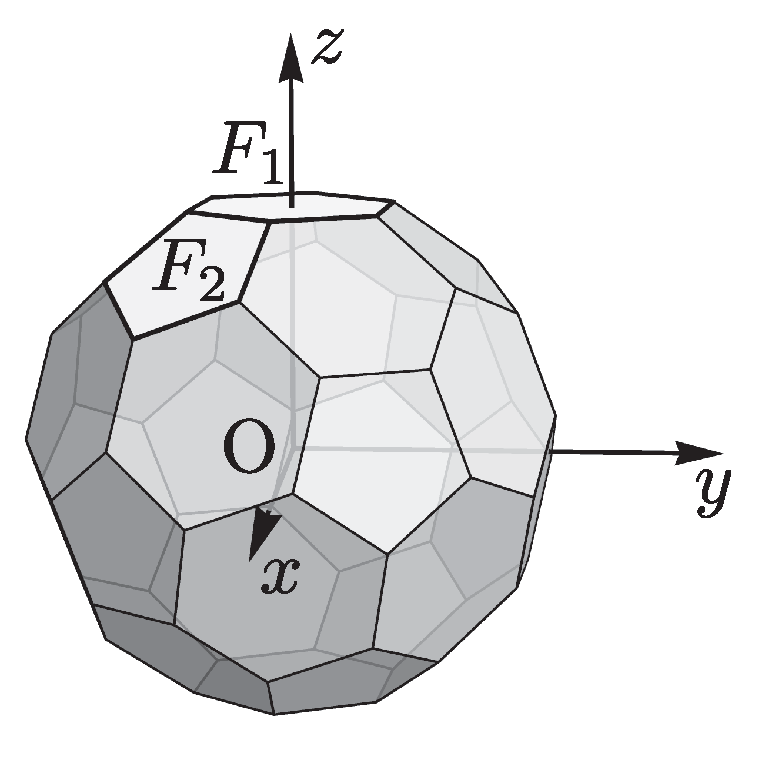
\includegraphics[width=0.5\textwidth]{axesAndFaces.pdf}
\caption{Coordinate axes and face labeling used in the Apple-Peel algorithm.
  The polyhedron is rotated so that the starting face $F_1$ lies at the
  ``north pole'' ($+z$ axis).}
\label{fig:axes}
\end{figure}

Let $\mathbf{c}_1$ be the centroid of the starting face $F_1$ (fixed throughout),
$\mathbf{c}_k$ the centroid of the current face $F_k$, and
$\mathbf{c}_j$ the centroid of a candidate adjacent face $F_j$.
We call $F_j$ a \textbf{right candidate} if
\begin{equation}
  \det(\mathbf{c}_1,\,\mathbf{c}_k,\,\mathbf{c}_j) \;\leq\; \varepsilon,
  \qquad \varepsilon = 10^{-10}.
  \label{eq:left}
\end{equation}
The right half-space consists of faces whose centroid lies clockwise
of the current direction when viewed from outside the polyhedron;
selecting from it enforces the CW spiral at every step
(Figure~\ref{fig:leftcond}).
The reference point $\mathbf{c}_1$ is the starting-face centroid and
remains \emph{fixed} at every step of the peeling sequence.
This \textbf{global} reference guarantees that the spiral direction
around the $z$-axis is consistent throughout; using the previous face
centroid $\mathbf{c}_{k-1}$ as a \emph{local} reference allows the
spiral direction to drift between steps and breaks the equivariance of
the algorithm under the symmetry group (see Remark~\ref{rem:symmetry3d}).
The threshold $\varepsilon=10^{-10}$ absorbs floating-point noise in the
determinant, which arises for solids with irrational coordinates
(e.g., the Dodecahedron, whose vertices involve the golden ratio)
and can cause $\det\approx 0$ values to flip sign across symmetry-equivalent pairs.

\begin{figure}[htbp]
\centering
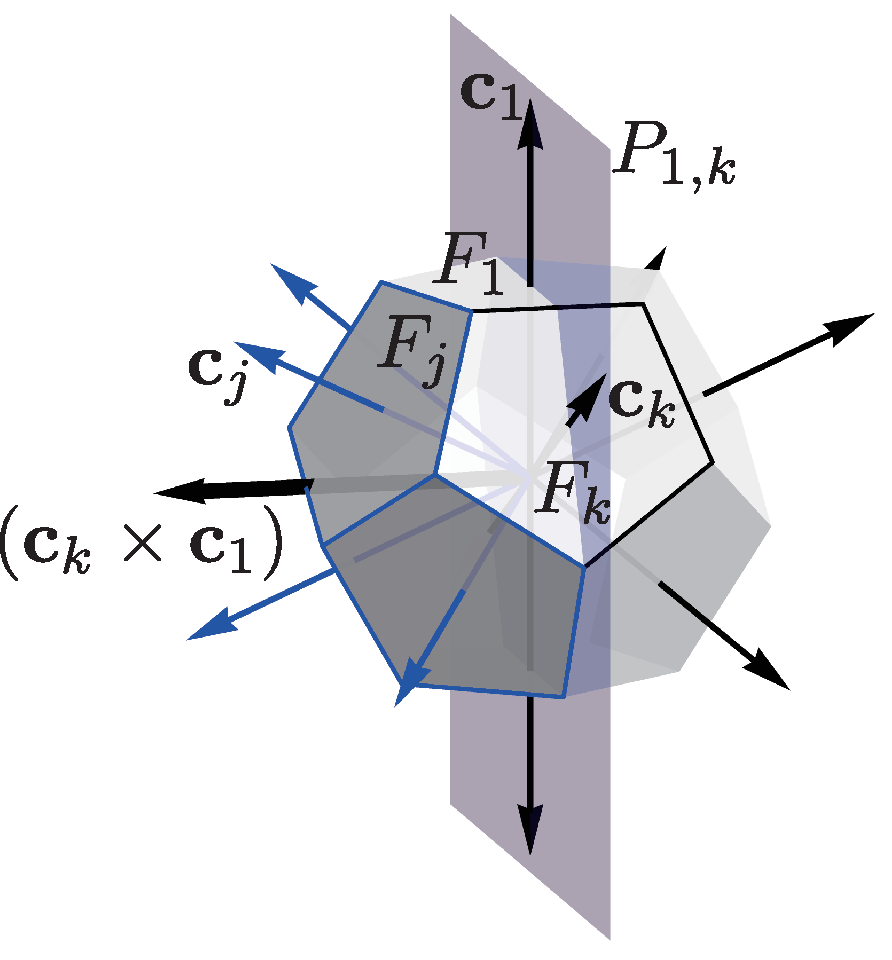
\includegraphics[width=0.55\textwidth]{leftside01.pdf}
\caption{Illustration of the right half-space condition~\eqref{eq:left}.
  $P_{1,k}$ denotes the plane through the origin spanned by
  $\mathbf{c}_1$ and $\mathbf{c}_k$, with normal $\mathbf{c}_k\times\mathbf{c}_1$.
  Blue arrows indicate the outward normal vectors of the candidate faces;
  dark gray faces are unvisited faces not yet in the peeling sequence.
  Candidate face $F_j$ is a right candidate if its centroid
  $\mathbf{c}_j$ lies in the half-space clockwise of $\mathbf{c}_k$
  when viewed from outside, i.e.\ on the $(\mathbf{c}_k\times\mathbf{c}_1)$ side of $P_{1,k}$.}
\label{fig:leftcond}
\end{figure}

The Darboux frame constructs a local coordinate system on the sphere
surface at the current face centroid.
It is used \emph{only} in the fallback branch of one of the two
selection rules (when no right candidate exists);
the rules themselves are introduced in Section~\ref{sec:rules}.

\begin{defn}[Darboux frame on the sphere]
\label{def:darboux}
Given consecutive face centroids $\mathbf{c}_{k-1}$ and $\mathbf{c}_k$,
define:
\begin{align}
  \hat{\mathbf{n}} &= \frac{\mathbf{c}_k}{\|\mathbf{c}_k\|},
  \label{eq:nhat}\\
  %\hat{\mathbf{f}} &= \mathrm{Normalize}\!\bigl(
  %             (\mathbf{c}_k - \mathbf{c}_{k-1})
  %             - [(\mathbf{c}_k - \mathbf{c}_{k-1})\cdot\hat{\mathbf{n}}]\,\hat{\mathbf{n}}
  %           \bigr),
 \hat{\mathbf{f}} &= \frac{
               (\mathbf{c}_k - \mathbf{c}_{k-1})
               - [(\mathbf{c}_k - \mathbf{c}_{k-1})\cdot\hat{\mathbf{n}}]\,\hat{\mathbf{n}}}{\left\|
               (\mathbf{c}_k - \mathbf{c}_{k-1})
               - [(\mathbf{c}_k - \mathbf{c}_{k-1})\cdot\hat{\mathbf{n}}]\,\hat{\mathbf{n}}
             \right\|},
  \label{eq:fhat}\\
  \hat{\mathbf{l}} &= \hat{\mathbf{n}} \times \hat{\mathbf{f}}.
  \label{eq:lhat}
\end{align}
Here $\hat{\mathbf{n}}$ is the sphere normal, $\hat{\mathbf{f}}$ is the forward direction
(projection of the step vector onto the tangent plane at $\mathbf{c}_k$),
and $\hat{\mathbf{l}}$ is the left direction.
\end{defn}

The \emph{signed angle} from the forward direction to a candidate $F_j$ is
\begin{equation}
  \varphi_j = \operatorname{atan2}\!\bigl(
    \tilde{\mathbf{c}}_j \cdot \hat{\mathbf{l}},\;
    \tilde{\mathbf{c}}_j \cdot \hat{\mathbf{f}}
  \bigr),
  \quad
  \tilde{\mathbf{c}}_j
    = \frac{\mathbf{c}_j - (\mathbf{c}_j\cdot\hat{\mathbf{n}})\hat{\mathbf{n}}}
           {\|\mathbf{c}_j - (\mathbf{c}_j\cdot\hat{\mathbf{n}})\hat{\mathbf{n}}\|}.
  \label{eq:phi}
\end{equation}
Here $\operatorname{atan2}(y,x)$ denotes the four-quadrant inverse tangent,
returning values in $(-\pi,\pi]$, so that $\varphi_j>0$ indicates a left turn
and $\varphi_j<0$ a right turn.

\subsection{Two Selection Rules}
\label{sec:rules}

Let $R$ denote the set of right candidates at the current step
and $P$ the full set of unvisited neighbors.
Note that $\det(\mathbf{c}_1,\mathbf{c}_k,\mathbf{c}_j)
= (\mathbf{c}_1\times\mathbf{c}_k)\cdot\mathbf{c}_j$,
so the right-candidate filter \eqref{eq:left} and the selection criterion below
both measure the same quantity: the signed volume spanned by
$\mathbf{c}_1$, $\mathbf{c}_k$, and the candidate.
Using the same global quantity for both filter and selection ensures
that the spiral direction is consistent across all steps.

We define two rules, named the \textbf{Spiral rule} (RS) and the
\textbf{Zonal rule} (RZ).

\begin{description}
  \item[\textbf{RS} (Spiral rule, min\,Det)]
    Select
    $\displaystyle\arg\min_{j\in R}\,\det(\mathbf{c}_1,\mathbf{c}_k,\mathbf{c}_j)$
    (most negative determinant $=$ sharpest clockwise spiral).
    Fallback when $R=\emptyset$:
    $\arg\min_{j\in P}\,\varphi_j$ via the Darboux frame
    (Definition~\ref{def:darboux});
    ties broken by $\arg\min_{j\in P}\,|\det(\mathbf{c}_1,\mathbf{c}_k,\mathbf{c}_j)|$.

  \item[\textbf{RZ} (Zonal rule, max\,$z$)]
    Select $\displaystyle\arg\max_{j\in R}\,(\mathbf{c}_j)_z$
    (highest centroid along the peeling axis);
    $z$-ties within $10^{-10}$ are broken by
    $\arg\min_{j\in R}\,\det(\mathbf{c}_1,\mathbf{c}_k,\mathbf{c}_j)$.
    Fallback when $R=\emptyset$:
    $\arg\min_{j\in P}\,(\mathbf{c}_j)_z$;
    $z$-ties broken by
    $\arg\min_{j\in P}\,\det(\mathbf{c}_1,\mathbf{c}_k,\mathbf{c}_j)$.
\end{description}

\begin{remark}[Rationale for rule names and criteria]
RS produces a tight clockwise coil around the $z$-axis by always taking the
most negative determinant (sharpest clockwise turn);
the path resembles a helix (spiral) descending from north pole to south pole.
RZ sweeps each latitude band in turn before descending to the next,
producing a zonal scan analogous to geographic latitude zones.

Using $\det(\mathbf{c}_1,\mathbf{c}_k,\mathbf{c}_j)$ as the primary RS
criterion---rather than the Darboux angle $\varphi_j$---aligns the selection
with the right-candidate filter (both use the same global reference $\mathbf{c}_1$),
and ensures equivariance under the symmetry group:
$\det(A\mathbf{c}_1,A\mathbf{c}_k,A\mathbf{c}_j)=\det(A)\,\det(\mathbf{c}_1,\mathbf{c}_k,\mathbf{c}_j)=\det(\mathbf{c}_1,\mathbf{c}_k,\mathbf{c}_j)$
for any $A\in\mathrm{SO}(3)$.
The Darboux frame $\varphi_j$ depends on the local step direction
$\mathbf{c}_{k-1}\to\mathbf{c}_k$ and uses a \emph{local} reference that
changes at every step; its use is retained only in the RS fallback branch
as a geometric tiebreaker when no right candidate exists.
For RZ, the $z$-tiebreak was previously also based on $\varphi_j$; it is
here replaced by $\det$, which is equivalent in practice and
formally consistent.
Algorithm~\ref{alg:peel} gives the complete procedure.
\end{remark}

\begin{algorithm}[tp]
\caption{Apple-Peel Unfolding (3D, rule $r \in \{\text{RS, RZ}\}$,
         variant $v \in \{\text{w},\text{n}\}$).
         variant w = with fallback; variant n = no fallback.}
\label{alg:peel}
\begin{algorithmic}[1]
\Require vertex coordinates, faces, adjacency lists,
         starting pair $(F_1,F_2)$, rule $r$, variant $v$
\Ensure face selection order, success flag
\State $\mathit{order} \gets [F_1,\,F_2]$;\;
       $\mathit{prev} \gets F_1$;\; $\mathit{last} \gets F_2$
\While{$\mathit{last}$ has unvisited adjacent faces}
  \State let $P$ = unvisited neighbors of $\mathit{last}$;\;
         $R \gets \{\,j\in P : \det(\mathbf{c}_1,\mathbf{c}_{\mathit{last}},\mathbf{c}_j)\le \varepsilon\,\}$
         \hfill\eqref{eq:left}
  \If{$R \neq \emptyset$}
    \If{$r = \text{RS}$}
      \State $\mathit{next} \gets \arg\min_{j\in R}\,\det(\mathbf{c}_1,\mathbf{c}_{\mathit{last}},\mathbf{c}_j)$
    \ElsIf{$r = \text{RZ}$}
      \State $\mathit{next} \gets \arg\max_{j\in R}\,(\mathbf{c}_j)_z$;\;
             $z$-ties broken by $\arg\min_j\,\det(\mathbf{c}_1,\mathbf{c}_{\mathit{last}},\mathbf{c}_j)$
    \EndIf
  \ElsIf{$v = \text{n}$} \Comment{no-fallback variant}
    \State \Return $(\mathit{order},\,\text{failure})$
  \Else \Comment{with-fallback variant: $R=\emptyset$, $v=\text{w}$}
    \If{$r = \text{RS}$}
      \State compute Darboux frame $(\hat{\mathbf{n}},\hat{\mathbf{f}},\hat{\mathbf{l}})$
             from $\mathbf{c}_{\mathit{prev}},\mathbf{c}_{\mathit{last}}$
             \hfill (Def.~\ref{def:darboux})
      \State $\mathit{next} \gets \arg\min_{j\in P}\,\varphi_j$;\;
             ties by $\arg\min_j\,|\det(\mathbf{c}_1,\mathbf{c}_{\mathit{last}},\mathbf{c}_j)|$
    \ElsIf{$r = \text{RZ}$}
      \State $\mathit{next} \gets \arg\min_{j\in P}\,(\mathbf{c}_j)_z$;\;
             $z$-ties by $\arg\min_j\,\det(\mathbf{c}_1,\mathbf{c}_{\mathit{last}},\mathbf{c}_j)$
    \EndIf
  \EndIf
  \State append $\mathit{next}$ to $\mathit{order}$;\;
         remove $\mathit{next}$ from all adjacency lists;\;
         $\mathit{prev} \gets \mathit{last}$;\;
         $\mathit{last} \gets \mathit{next}$
\EndWhile
\State \Return $\bigl(\mathit{order},\;|\mathit{order}| = |\mathit{faces}|\bigr)$
\end{algorithmic}
\end{algorithm}


\begin{figure}[htbp]
\centering
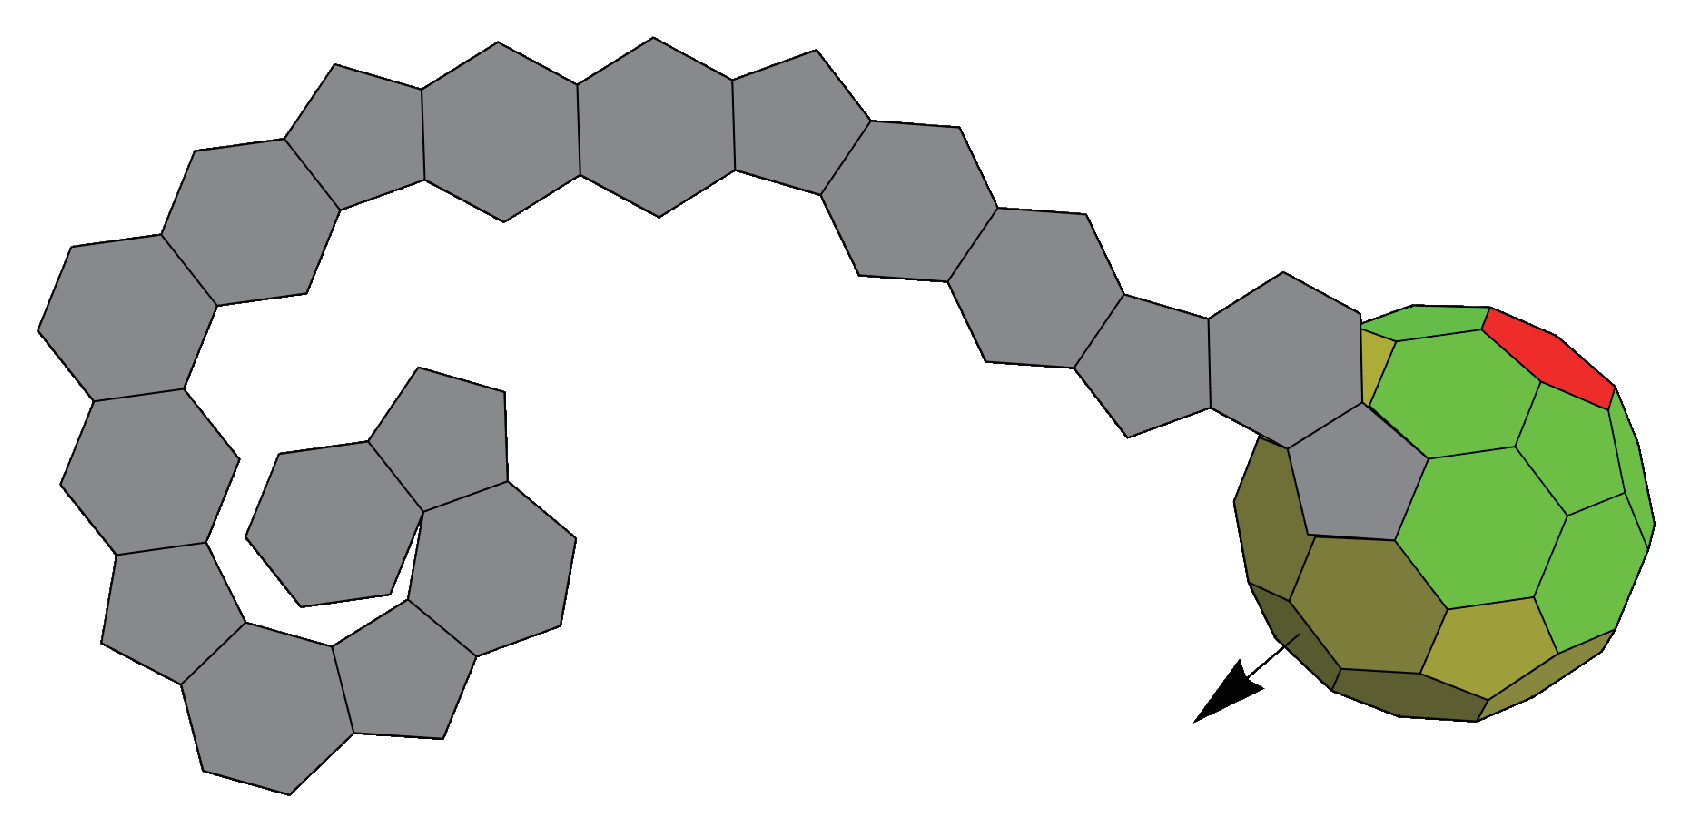
\includegraphics[width=0.8\textwidth]{exampleOfPeeling.pdf}
\caption{Apple-Peel unfolding of the Truncated Icosahedron under RZ (max\,$z$),
  shown after 19 of 32 faces have been selected.
  Gray faces (left) show the unfolded net of the faces peeled so far,
  laid flat by unfolding each consecutive pair of faces along their shared edge.
  On the Truncated Icosahedron (right), olive faces have been peeled and
  green faces remain; the red face is the last face in the sequence,
  which coincides with the antipode of $F_1$ under RZ\@.
  The arrow indicates the direction of $\mathbf{c}_1$.}
\label{fig:peel-example}
\end{figure}

% ============================================================
\subsection{Net Construction from Selection Order}
\label{sec:netconstruct}
% ============================================================

Given a successful selection order $[F_1,\ldots,F_n]$ produced by
Algorithm~\ref{alg:peel}, a flat 2D net is obtained by sequentially
folding the accumulated strip of faces into the plane of the next face,
using the shared edge as a hinge.
Because $F_k$ ($k\ge2$) is always selected from the unvisited neighbors
of $F_{k-1}$, consecutive faces share exactly one edge.
Figure~\ref{fig:peel-example} shows this process in progress for the
truncated icosahedron after 19 of its 32 faces have been selected.

Let $\mathbf{n}_i$ denote the outward unit normal of face $F_i$.
At step $k$, the faces $F_1,\ldots,F_{k-1}$ (already coplanar after the
previous step) are rotated by the exterior dihedral angle
$\theta_k = \arccos(\mathbf{n}_{k-1}\cdot\mathbf{n}_k)$ around the shared
edge $F_{k-1}\cap F_k$, bringing the strip into $F_k$'s plane.
The rotation axis $\mathbf{a}_k = (\mathbf{n}_{k-1}\times\mathbf{n}_k)/\|\mathbf{n}_{k-1}\times\mathbf{n}_k\|$
is parallel to the shared edge.
After all $n$ steps the entire strip lies in $F_n$'s plane and is
projected to 2D.
Algorithm~\ref{alg:net2d} gives the complete procedure.

\begin{algorithm}[htbp]
\caption{2D Net Construction (3D polyhedra)}
\label{alg:net2d}
\begin{algorithmic}[1]
\Require vertex coordinates $\mathit{vers}$ (3D), face list $\mathit{faces}$,
         selection order $[F_1,\ldots,F_n]$
\Ensure 2D polygon list $\mathit{net} = [\Pi_1,\ldots,\Pi_n]$
\State Compute outward unit normal $\mathbf{n}_i$ for each face $F_i$
       \hfill\Comment{$\mathbf{n}_i \propto (v_2-v_1)\times(v_3-v_1)$, oriented so $\mathbf{n}_i\cdot\bar{v}_i>0$}
\State $S \gets [\,]$ \hfill\Comment{accumulates 3D vertex arrays of placed faces}
\For{$k \gets 2$ \textbf{to} $n$}
  \State Append vertex array of $F_{k-1}$ (original 3D coordinates) to $S$
  \State $\{u,w\} \gets \mathit{faces}[F_{k-1}]\cap \mathit{faces}[F_k]$
         \hfill\Comment{shared edge (hinge)}
  \State $\mathbf{a} \gets \mathrm{Normalize}(\mathbf{n}_{k-1}\times\mathbf{n}_k)$
         \hfill\Comment{rotation axis, parallel to shared edge}
  \State $\theta \gets \arccos\!\bigl(\mathrm{Clip}(\mathbf{n}_{k-1}\cdot\mathbf{n}_k,\,[-1,1])\bigr)$
         \hfill\Comment{exterior dihedral angle}
  \State Rotate every vertex in $S$ by $\theta$ around axis $\mathbf{a}$ through $\mathit{vers}[u]$
         \hfill\Comment{brings strip $F_1\ldots F_{k-1}$ coplanar with $F_k$}
\EndFor
\State Append vertex array of $F_n$ (original 3D coordinates) to $S$
\State Let $R$ be the rotation mapping $\mathbf{n}_n$ to $+z$
\State $\mathbf{p}[v] \gets (R\,v)_{xy}$ for each vertex $v$ in $S$
       \hfill\Comment{project to 2D}
\State Rotate all $\mathbf{p}$ so that $\mathbf{p}[\mathbf{c}_2]-\mathbf{p}[\mathbf{c}_1]$
       aligns with $+x$
       \hfill\Comment{canonical orientation}
\State \Return $\bigl[[\mathbf{p}[v]:v\!\in\! F_k]\;:\;k=1,\ldots,n\bigr]$
\end{algorithmic}
\end{algorithm}

% ============================================================
\section{Results: 3D Polyhedra}
\label{sec:3d}
% ============================================================

We classify each polyhedron according to the fraction of starting pairs
$(F_1,F_2)$ that yield a successful net under the best available rule:
\emph{Perfect} if every pair succeeds,
\emph{Possible} if at least one pair succeeds, and
\emph{Impossible} if no pair succeeds.
The same classification is used for 4D polytopes in
Section~\ref{sec:4d}.

\subsection{Platonic Solids}

Both RS and RZ achieve 100\% success on all five Platonic solids
with the fallback branch active, classifying each as \emph{Perfect}.
The uniform outcome across all starting pairs is a consequence of
equivariance under the face-transitive rotation group: if the algorithm
is equivariant, the success rate must be either 0\% or 100\% for
each solid (Remark~\ref{rem:symmetry3d}).
Figure~\ref{fig:platonic-nets} shows a representative net for each solid.

\begin{figure}[htbp]
\centering
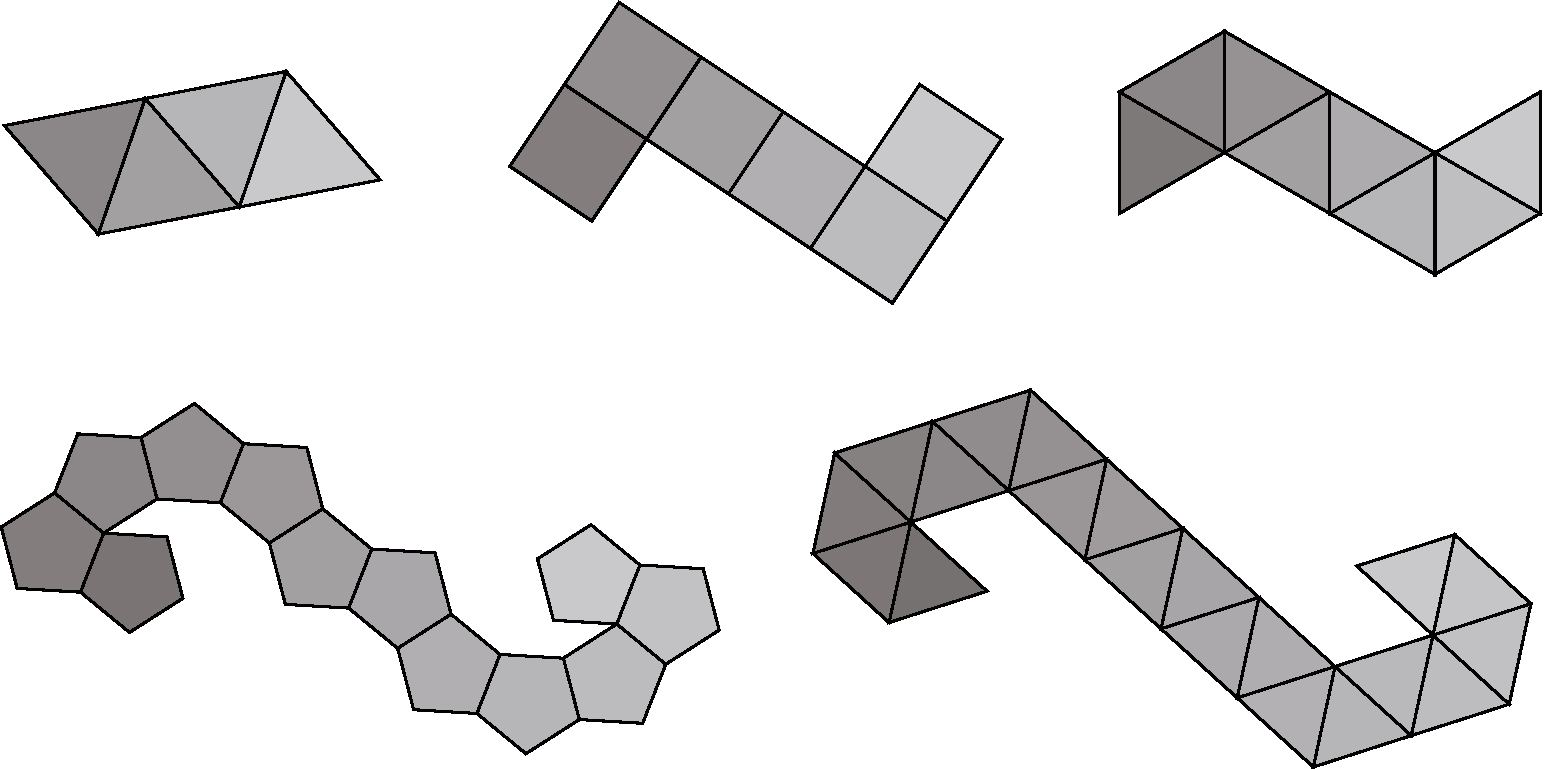
\includegraphics[width=\textwidth]{PlatonicNets.pdf}
\caption{Nets of the five Platonic solids obtained by
  Apple-Peel Unfolding (both RS and RZ rules produce identical nets for
  each solid).
  Face shading indicates the selection order:
  dark (first face $F_1$) through light (last face $F_n$).
  By equivariance, all successful orderings of a given solid produce
  congruent nets.}
\label{fig:platonic-nets}
\end{figure}

\begin{remark}[Symmetry and equivariance for Platonic solids]
\label{rem:symmetry3d}
Each Platonic solid is face-transitive: the rotation group $G$ maps any
ordered adjacent face pair $(F_1, F_2)$ to any other.
If the algorithm is \emph{equivariant}---meaning a symmetry $\sigma\in G$
maps the selection sequence for $(F_1,F_2)$ to the sequence for
$(\sigma F_1, \sigma F_2)$---then every pair has the same success or
failure outcome, so the success rate must be 0\% or 100\%.

To see why the global right condition \eqref{eq:left} achieves equivariance,
let $A$ be the composite rotation $\mathrm{FaceUp}(\sigma F_1)\circ\sigma\circ\mathrm{FaceUp}(F_1)^{-1}$,
so that transformed centroids satisfy $\mathbf{c}'_j = A\mathbf{c}_j$.
Because $A$ is a proper rotation, $\det(A)=1$, and therefore
\[
  \det(\mathbf{c}'_1,\mathbf{c}'_k,\mathbf{c}'_j)
  = \det(A)\,\det(\mathbf{c}_1,\mathbf{c}_k,\mathbf{c}_j)
  = \det(\mathbf{c}_1,\mathbf{c}_k,\mathbf{c}_j).
\]
The right-candidate set is thus the image of the original set under the
label permutation induced by $\sigma$.
For RS, the primary selection criterion $\det(\mathbf{c}_1,\mathbf{c}_k,\mathbf{c}_j)$
is invariant under $A$, so the $\arg\min$ selection is likewise equivariant.
The $z$-coordinate (RZ primary) and the Det tiebreak are both preserved by $A$
since $A$ is a proper rotation.
Hence both rules are equivariant in this case.

In contrast, in general cases a \emph{local} reference $\mathbf{c}_{k-1}$ would transform
as $A\mathbf{c}_{k-1}$ together with the other centroids, but the
composite rotation $A$ depends on $(F_1,\sigma)$ and changes between
symmetry-equivalent steps, destroying the compatibility of the
left-candidate sets.

Two further implementation details are required for exact equivariance:
\begin{enumerate}[nosep]
  \item \emph{Epsilon threshold.}
    For the Dodecahedron (golden-ratio coordinates), finite-precision
    arithmetic causes $\det(\mathbf{c}_1,\mathbf{c}_k,\mathbf{c}_j)\approx 0$
    values to fluctuate by $\sim 10^{-16}$.
    The threshold $\varepsilon=10^{-10}$ prevents sign-flips that would
    classify the same candidate as left for one pair but right for a
    symmetry-equivalent pair.
  \item \emph{Geometric tie-breaks.}
    Any ties after the primary criterion are resolved by a geometric
    secondary criterion rather than by face index.
    For RS, the primary criterion is $\arg\min_j\,\det(\mathbf{c}_1,\mathbf{c}_k,\mathbf{c}_j)$;
    exact ties use $\arg\min_j\,|\det(\mathbf{c}_1,\mathbf{c}_k,\mathbf{c}_j)|$.
    For RZ, $z$-ties are broken by $\arg\min_j\,\det(\mathbf{c}_1,\mathbf{c}_k,\mathbf{c}_j)$.
    Each Det value satisfies
    $\det(A\mathbf{a},A\mathbf{b},A\mathbf{c})=\det(\mathbf{a},\mathbf{b},\mathbf{c})$
    for $A\in\mathrm{SO}(3)$, so equivariance is preserved at every level.
    A tie-break by face index (list order) would depend on the arbitrary
    labeling of faces and violate equivariance.
    This Det-based convention is the direct 3D analogue of the tie-break
    adopted in the 4D extension (Section~\ref{sec:4dresults}).
    Verification on all five Platonic solids and thirteen Archimedean solids
    confirms that exact Det ties are never triggered in practice;
    the criterion serves as a formal safeguard for completeness.
\end{enumerate}

\end{remark}

\begin{remark}[Strict right condition ($\varepsilon<0$) as a formal variant]
\label{rem:strict-eps}
The standard threshold $\det(\mathbf{c}_1,\mathbf{c}_k,\mathbf{c}_j)\le \varepsilon$
(with $\varepsilon=10^{-10}$, i.e.\ $\varepsilon>0$) admits faces whose
determinant is near zero---those whose centroid lies approximately in the
meridian plane spanned by $\mathbf{c}_1$ and $\mathbf{c}_k$.
Geometrically, such a face lies ``due south'' along the current meridian
and thus neither turns the spiral clockwise nor counterclockwise.

We also tested the \emph{strict} variant $\varepsilon<0$, i.e.\
thresh $= -10^{-10}$, which excludes these boundary faces from
the right-candidate set $R$ and sends them to the fallback branch.
Table~\ref{tab:strict} summarizes the results for the Spiral rule (RS)
and Zonal rule (RZ) on all five Platonic solids.

\begin{table}[ht]
\centering
\caption{Success rates under the strict right condition
  (thresh $=-10^{-10}$, i.e.\ $\varepsilon<0$) for the Spiral rule (RS)
  and Zonal rule (RZ) on all five Platonic solids.
  RS(w)/RZ(w) = with fallback; RS(n)/RZ(n) = without fallback.}
\label{tab:strict}
\renewcommand{\arraystretch}{1.1}
\begin{tabular}{llrrrrr}
\toprule
Solid & $\{p,q\}$ & Pairs & RS(w) & RS(n) & RZ(w) & RZ(n) \\
\midrule
Tetrahedron  & $\{3,3\}$ & 12 & 100\% & 100\% & 100\% & 100\% \\
Cube         & $\{4,3\}$ & 24 & 100\% &   0\% & 100\% &   0\% \\
Octahedron   & $\{3,4\}$ & 24 & 100\% &   0\% & 100\% &   0\% \\
Dodecahedron & $\{5,3\}$ & 60 & 100\% &   0\% & 100\% &   0\% \\
Icosahedron  & $\{3,5\}$ & 60 & 100\% &   0\% & 100\% &   0\% \\
\bottomrule
\end{tabular}
\end{table}

Three observations:
\begin{enumerate}[nosep]
  \item \emph{Equivariance is preserved.}
    All entries are 0\% or 100\%, confirming that the strict condition is
    also equivariant (the determinant inequality is preserved under proper
    rotations regardless of the sign of the threshold).
  \item \emph{With fallback: 100\% for all solids.}
    The ``due south'' faces excluded from $L$ are redirected to the fallback
    branch.  The RS fallback ($\arg\min\varphi_j$) and the RZ fallback
    ($\arg\min z$) both select these faces via a different criterion, so the
    same peeling sequence is ultimately produced.
  \item \emph{Without fallback: 100\% only for the Tetrahedron.}
    The Tetrahedron has no face whose centroid lies exactly in the meridian
    plane after Face-up alignment, so the strict condition causes no
    additional terminations.  For all other Platonic solids there exists at
    least one step where the sole viable candidate has $\det\approx 0$; the
    strict condition empties $L$ at that step and the no-fallback variant
    terminates immediately.
\end{enumerate}
The standard $\varepsilon>0$ setting is therefore preferred: it is the
unique choice that (a) preserves equivariance and (b) maximizes the
success rate without fallback.
\end{remark}

\paragraph{Dodecahedron.}
The Dodecahedron (12 pentagonal faces) achieves 100\% success under
both RS and RZ with the fallback branch active.
Under the strict no-fallback variant ($\varepsilon<0$), the success
rate drops to 0\% for all Platonic solids except the Tetrahedron
(Table~\ref{tab:strict}).

RS takes the sharpest available right turn at each step, wrapping the
path clockwise around the surface and reaching the opposite pole in all
60 starting pairs.

Kaino \cite{Kaino2019} illustrates two net types for the Dodecahedron
(``Dodecahedron~1'' and ``Dodecahedron~2'' in Fig.~1 of that work).
The Apple-Peel algorithm under both RS and RZ produces only
``Dodecahedron~2''; ``Dodecahedron~1'' does not arise under the
right-half-space spiral constraint, indicating that the Apple-Peel
family does not exhaust all net topologies of the Dodecahedron.

\subsection{Archimedean Solids}

The Archimedean solid experiments apply the same Face-up pre-rotation
as the Platonic solid computations: the solid is rotated so that the
centroid of the first face $F_1$ aligns with the $+z$ axis before
running the algorithm.
The equal azimuthal spacing of Remark~\ref{rem:symmetry3d} does not
apply here because Archimedean solids lack the full face-transitive
symmetry of Platonic solids; however, the Face-up condition ensures
that comparisons across rules are made on a consistent geometric footing.

\begin{table}[ht]
\centering
\caption{Unfolding success rates (\%) on the 13 Archimedean solids.
  ``w'' = with fallback; ``n'' = no fallback.
  Bold entries mark the best result per row.}
\label{tab:archimedean}
\renewcommand{\arraystretch}{1.2}
\small\setlength{\tabcolsep}{4pt}
\begin{tabular}{llrrrrrr}
\toprule
& & & & \multicolumn{2}{c}{RS\,(\%)} & \multicolumn{2}{c}{RZ\,(\%)} \\
\cmidrule(lr){5-6}\cmidrule(lr){7-8}
Polyhedron & v.c. & $F$ & Pairs & w & n & w & n \\
\midrule
Truncated Tetrahedron        & 3.6.6       &  8 &  36 & \textbf{66.7} & \textbf{66.7} & 33.3 & 33.3 \\
Cuboctahedron                & 3.4.3.4     & 14 &  48 &  0.0 &  0.0 &  0.0 &  0.0 \\
Truncated Cube               & 3.8.8       & 14 &  72 &  0.0 &  0.0 &  0.0 &  0.0 \\
Truncated Octahedron         & 4.6.6       & 14 &  72 & 41.7 & 41.7 & \textbf{100.0} & \textbf{100.0} \\
Rhombicuboctahedron          & 3.4.4.4     & 26 &  96 &  0.0 &  0.0 &  0.0 &  0.0 \\
Truncated Cuboctahedron      & 4.6.8       & 26 & 144 &  0.0 &  0.0 & \textbf{100.0} & \textbf{100.0} \\
Snub Cube                    & 3.3.3.3.4   & 38 & 120 & 20.0 &  0.0 & \textbf{40.0} & 20.0 \\
Icosidodecahedron            & 3.5.3.5     & 32 & 120 &  0.0 &  0.0 &  0.0 &  0.0 \\
Truncated Dodecahedron       & 3.10.10     & 32 & 180 &  0.0 &  0.0 &  0.0 &  0.0 \\
Truncated Icosahedron        & 5.6.6       & 32 & 180 &  0.0 &  0.0 & \textbf{100.0} & \textbf{100.0} \\
Rhombicosidodecahedron       & 3.4.5.4     & 62 & 240 &  0.0 &  0.0 &  0.0 &  0.0 \\
Truncated Icosidodecahedron  & 4.6.10      & 62 & 360 &  0.0 &  0.0 & \textbf{66.7} & \textbf{66.7} \\
Snub Dodecahedron            & 3.3.3.3.5   & 92 & 300 &  0.0 &  0.0 &  0.0 &  0.0 \\
\bottomrule
\end{tabular}
\end{table}

\paragraph{Observations.}
\begin{itemize}
  \item \textbf{Seven of thirteen solids (54\%) yield 0\% under both RS and RZ},
        concentrated among those with many square faces (cuboctahedron,
        truncated cube, rhombicuboctahedron, icosidodecahedron,
        truncated dodecahedron, rhombicosidodecahedron, snub dodecahedron).
  \item \textbf{RZ achieves 100\% on three solids}:
        truncated octahedron, truncated cuboctahedron, and
        truncated icosahedron; it also achieves the best
        result on the truncated icosidodecahedron (66.7\%).
        RS achieves its highest rate on the truncated tetrahedron (66.7\%)
        and remains positive only on two further solids:
        truncated octahedron (41.7\%) and snub cube (20.0\%).
  \item \textbf{RZ outperforms RS on four solids.}
        Truncated octahedron (RZ\,100\% $>$ RS\,41.7\%),
        truncated cuboctahedron (RZ\,100\% $>$ RS\,0\%),
        truncated icosahedron (RZ\,100\% $>$ RS\,0\%),
        truncated icosidodecahedron (RZ\,66.7\% $>$ RS\,0\%).
        RS outperforms RZ only on the truncated tetrahedron
        (RS\,66.7\% $>$ RZ\,33.3\%).
  \item \textbf{Fallback is essential only for the Snub Cube.}
        Removing the fallback leaves 12 of 13 solids unchanged.
        For the snub cube: RS drops from 20.0\% (24/120) to 0\%,
        and RZ drops from 40.0\% (48/120) to 20.0\% (24/120).
  \item \textbf{Mirror symmetry: counts preserved.}
        For all 13 Archimedean solids, running the algorithm on the mirror
        image (reflection $(x,y,z)\mapsto(-x,y,z)$) yields identical success
        counts for RZ (verified; Section~\ref{sec:mirror}).
        For the chiral snub cube, the successful $(F_1,F_2)$ pairs differ
        between original and mirror image under RZ, revealing sensitivity
        to chirality at the orbit level.
\end{itemize}

\paragraph{Structural interpretation.}
The results across thirteen Archimedean solids support the following
structural principles:
\begin{description}
  \item[Face-type uniformity and RZ dominance]
    The three solids achieving 100\% under RZ (truncated octahedron,
    truncated cuboctahedron, truncated icosahedron) all combine hexagonal
    faces with one or two other regular polygon types; the truncated
    icosidodecahedron reaches 66.7\% under RZ and shares the same
    hexagonal-face structure.
    The latitude-band structure of hexagonal solids is well-suited to
    the max-$z$ criterion, which sweeps each band in turn.
    By contrast, RS (min-Det) takes the sharpest available clockwise turn
    at each step, which can navigate around the hexagonal bands in some
    configurations but follows a more irregular path that not all
    starting pairs can complete successfully.
    The seven solids yielding 0\% under both rules contain squares in large
    proportions, which disrupt the right-condition filtering.

  \item[RS outperformance: Truncated Tetrahedron]
    This is the only Archimedean solid where RS (66.7\%) strictly outperforms
    RZ (33.3\%).
    Its 8-face structure (4 triangles + 4 hexagons) with only 36 pairs is
    the smallest Archimedean case; the sharpest-turn criterion navigates
    the alternating face types more reliably than the latitude criterion.

  \item[Path geometry: RZ on the Truncated Icosahedron]
    RZ achieves 100\% and produces a smooth band-by-band traversal through
    consecutive hexagons at the same latitude before descending.
    RS is unsuccessful on this solid with the Det-based criterion.
    A representative RZ sequence is shown in Section~\ref{sec:ex-ti}.
\end{description}
Figure~\ref{fig:arch-all} shows representative nets for four of the six successful Archimedean solids under RZ\@;
the Truncated Icosahedron and Snub Cube are treated separately in
Sections~\ref{sec:ex-ti} and~\ref{sec:ex-snub}.
\begin{figure}[htbp]
\centering
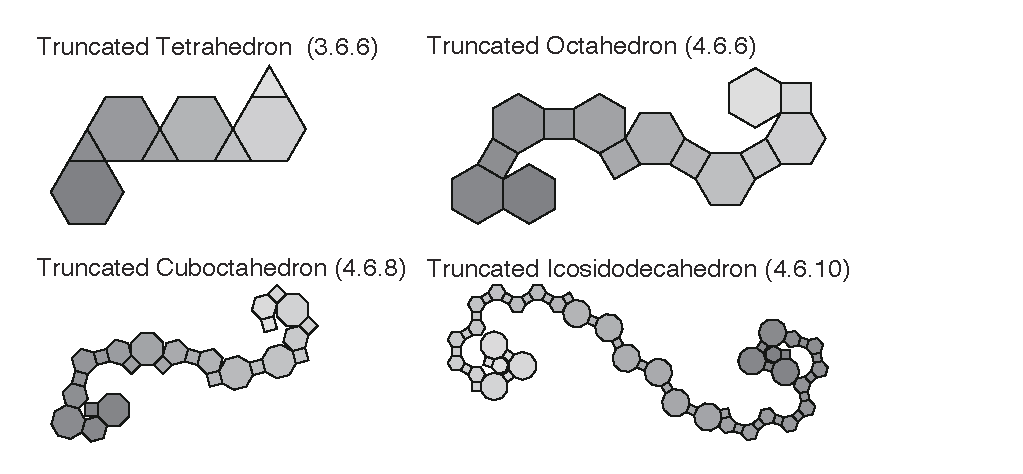
\includegraphics[width=\textwidth]{allExamples2.pdf}
\caption{Successful nets for four Archimedean solids: Truncated Tetrahedron
  (3.6.6, shown under RZ; RS achieves a higher rate of 66.7\%),
  Truncated Octahedron (4.6.6, RZ), Truncated Cuboctahedron (4.6.8, RZ),
  and Truncated Icosidodecahedron (4.6.10, RZ).
  Solids with all-zero success rates (7 of 13) are omitted;
  the Truncated Icosahedron and Snub Cube are discussed in
  Sections~\ref{sec:ex-ti} and~\ref{sec:ex-snub}.}
\label{fig:arch-all}
\end{figure}

\begin{figure}[htbp]
\centering
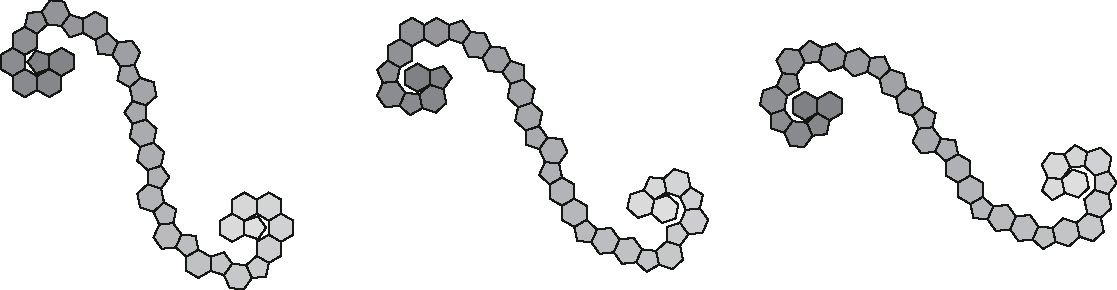
\includegraphics[width=0.9\textwidth]{11Nets.pdf}
\caption{Three representative nets of the Truncated Icosahedron under
  the Zonal rule (RZ, max\,$z$).
  Each net traverses the hexagonal faces band by band from north to south.}
\label{fig:ti-nets}
\end{figure}

% ------------------------------------------------------------
\subsection{Mirror Symmetry and Chirality Detection}
\label{sec:mirror}
% ------------------------------------------------------------

A reflection $\rho\colon (x,y,z)\mapsto(-x,y,z)$ maps each polyhedron to
its mirror image.
Because $\det(\rho)=-1$, the right half-space condition reverses sign:
$\det(\mathbf{c}_1,\mathbf{c}_k,\mathbf{c}_j)\le \varepsilon$ becomes
$-\det(\mathbf{c}_1,\mathbf{c}_k,\mathbf{c}_j)\le \varepsilon$.
Running the right-spiral algorithm on the mirror image is therefore equivalent
to running a \emph{left}-spiral algorithm on the original polyhedron.

\paragraph{Empirical check.}
We ran RS and RZ on both the original and the mirror image of all 13
Archimedean solids. The results are summarized in
Table~\ref{tab:mirror}; for all 13 solids the counts match exactly.

\begin{table}[ht]
\centering
\caption{Success counts for original vs.\ mirror image (all 13 Archimedean
  solids).  RZ counts were verified computationally;
  RS counts are inferred from the equivariance argument for the
  11 amphichiral solids and from the orbit-exchange behavior
  (analogous to RZ; cf.\ Section~\ref{sec:ex-snub})
  for the chiral snub cube.
  Counts are identical in every case.
  Numbers in parentheses indicate the count of geometrically distinct
  net types (equivariance classes of starting pairs);
  $-$ indicates zero successes.}
\label{tab:mirror}
\small
\setlength{\tabcolsep}{5pt}
\begin{tabular}{llrrrrr}
\toprule
Solid & v.c. & Pairs & \multicolumn{2}{c}{RS} & \multicolumn{2}{c}{RZ} \\
\cmidrule(lr){4-5}\cmidrule(lr){6-7}
 & & & Orig & Mirror & Orig & Mirror \\
\midrule
Truncated Tetrahedron       & 3.6.6       &  36 & 24\,(2) & 24\,(2) & 12\,(1) & 12\,(1) \\
Cuboctahedron               & 3.4.3.4     &  48 & \multicolumn{1}{c}{-} & \multicolumn{1}{c}{-} & \multicolumn{1}{c}{-} & \multicolumn{1}{c}{-} \\
Truncated Cube              & 3.8.8       &  72 & \multicolumn{1}{c}{-} & \multicolumn{1}{c}{-} & \multicolumn{1}{c}{-} & \multicolumn{1}{c}{-} \\
Truncated Octahedron        & 4.6.6       &  72 & 30\,(4) & 30\,(4) & 72\,(3) & 72\,(3) \\
Rhombicuboctahedron         & 3.4.4.4     &  96 & \multicolumn{1}{c}{-} & \multicolumn{1}{c}{-} & \multicolumn{1}{c}{-} & \multicolumn{1}{c}{-} \\
Truncated Cuboctahedron     & 4.6.8       & 144 & \multicolumn{1}{c}{-} & \multicolumn{1}{c}{-} &144\,(6) &144\,(6) \\
Snub Cube$^*$               & 3.3.3.3.4   & 120 & 24\,(1) & 24\,(1) & 48\,(2) & 48\,(2) \\
Icosidodecahedron           & 3.5.3.5     & 120 & \multicolumn{1}{c}{-} & \multicolumn{1}{c}{-} & \multicolumn{1}{c}{-} & \multicolumn{1}{c}{-} \\
Truncated Dodecahedron      & 3.10.10     & 180 & \multicolumn{1}{c}{-} & \multicolumn{1}{c}{-} & \multicolumn{1}{c}{-} & \multicolumn{1}{c}{-} \\
Truncated Icosahedron       & 5.6.6       & 180 & \multicolumn{1}{c}{-} & \multicolumn{1}{c}{-} &180\,(3) &180\,(3) \\
Rhombicosidodecahedron      & 3.4.5.4     & 240 & \multicolumn{1}{c}{-} & \multicolumn{1}{c}{-} & \multicolumn{1}{c}{-} & \multicolumn{1}{c}{-} \\
Truncated Icosidodecahedron & 4.6.10      & 360 & \multicolumn{1}{c}{-} & \multicolumn{1}{c}{-} &240\,(4) &240\,(4) \\
Snub Dodecahedron$^*$       & 3.3.3.3.5   & 300 & \multicolumn{1}{c}{-} & \multicolumn{1}{c}{-} & \multicolumn{1}{c}{-} & \multicolumn{1}{c}{-} \\
\bottomrule
\multicolumn{7}{l}{\small$^*$ Chiral solid (enantiomorphic pair).}
\end{tabular}
\end{table}

\paragraph{Amphichiral solids.}
For the 11 amphichiral solids, the mirror image is congruent to the
original under a proper rotation; equivariance then implies identical
counts.

\paragraph{Chiral solids.}
The two chiral solids require separate analysis.
The snub dodecahedron yields 0\% in both cases, so the counts agree
trivially.
For the snub cube, the counts agree but the successful \emph{pairs} differ;
the orbit-exchange structure is examined in Section~\ref{sec:ex-snub}.

% ------------------------------------------------------------
\subsection{Truncated Icosahedron: Hexagonal-Band Path under RZ}
\label{sec:ex-ti}
% ------------------------------------------------------------

The truncated icosahedron (soccer-ball pattern; 32 faces: 12 pentagons
and 20 hexagons) achieves 100\% success under RZ (all 180 starting pairs),
while RS (min-Det) yields 0\% on this solid.
This contrast illustrates how the two criteria navigate the hexagonal
latitude-band structure differently.

We denote each face type as $\mathtt{P}$ (pentagon) or $\mathtt{H}$
(hexagon).

\medskip
\noindent\textbf{RZ} (max\,$z$; representative starting pair, success 32/32):

\smallskip
\noindent\small
\textit{Types:} \texttt{P H H H H H P H P H H P H H P H H P H P H H P H P H P H P H H P}
\normalsize

The RZ path keeps longer runs of hexagonal faces (mean maximum consecutive
run $\approx 4.1$), traversing several consecutive hexagons at roughly the
same latitude before descending to the next ring---a \textbf{zonal band-by-band traversal}
around the peeling axis.
All 180 starting pairs succeed under RZ, confirming that the
max-$z$ criterion is compatible with the solid's hexagonal
latitude-band geometry.
Figure~\ref{fig:ti-nets} shows a sample of the resulting nets.

% ------------------------------------------------------------
\subsection{Snub Cube: Equivariance and Chiral Structure}
\label{sec:ex-snub}
% ------------------------------------------------------------

The snub cube (38 faces: 32 triangles and 6 squares) provides an
example where the success rates are partial and differ between rules:
RZ achieves 48 of 120 pairs (40.0\%) while RS achieves 24 of 120 (20.0\%).
The fallback branch is essential for this solid: removing it reduces
RS from 20.0\% to 0\% and RZ from 40.0\% to 20.0\%.

The 32 triangles decompose into two sub-orbits under the chiral
octahedral group $O$ (order 24): 24 \emph{snub} triangles (each sharing
one edge with a square) and 8 \emph{gyrate} triangles (sharing no edge
with a square).
Within each sub-orbit, every pair succeeds or fails uniformly under RZ,
confirming equivariance; the mixed outcome at the face-type level
reflects the distinct geometry of the two sub-orbits, not numerical
inconsistency.
Figure~\ref{fig:snub-nets} shows representative nets for each successful
orbit type under both chiralities:
(a)~Original, $F_1{=}\mathrm{snub}\,\triangle$;
(b)~Original, $F_1{=}\mathrm{gyrate}\,\triangle$;
(c)~Mirror, $F_1{=}\mathrm{snub}\,\triangle$;
(d)~Mirror, $F_1{=}\square$.

\begin{figure}[htbp]
\centering
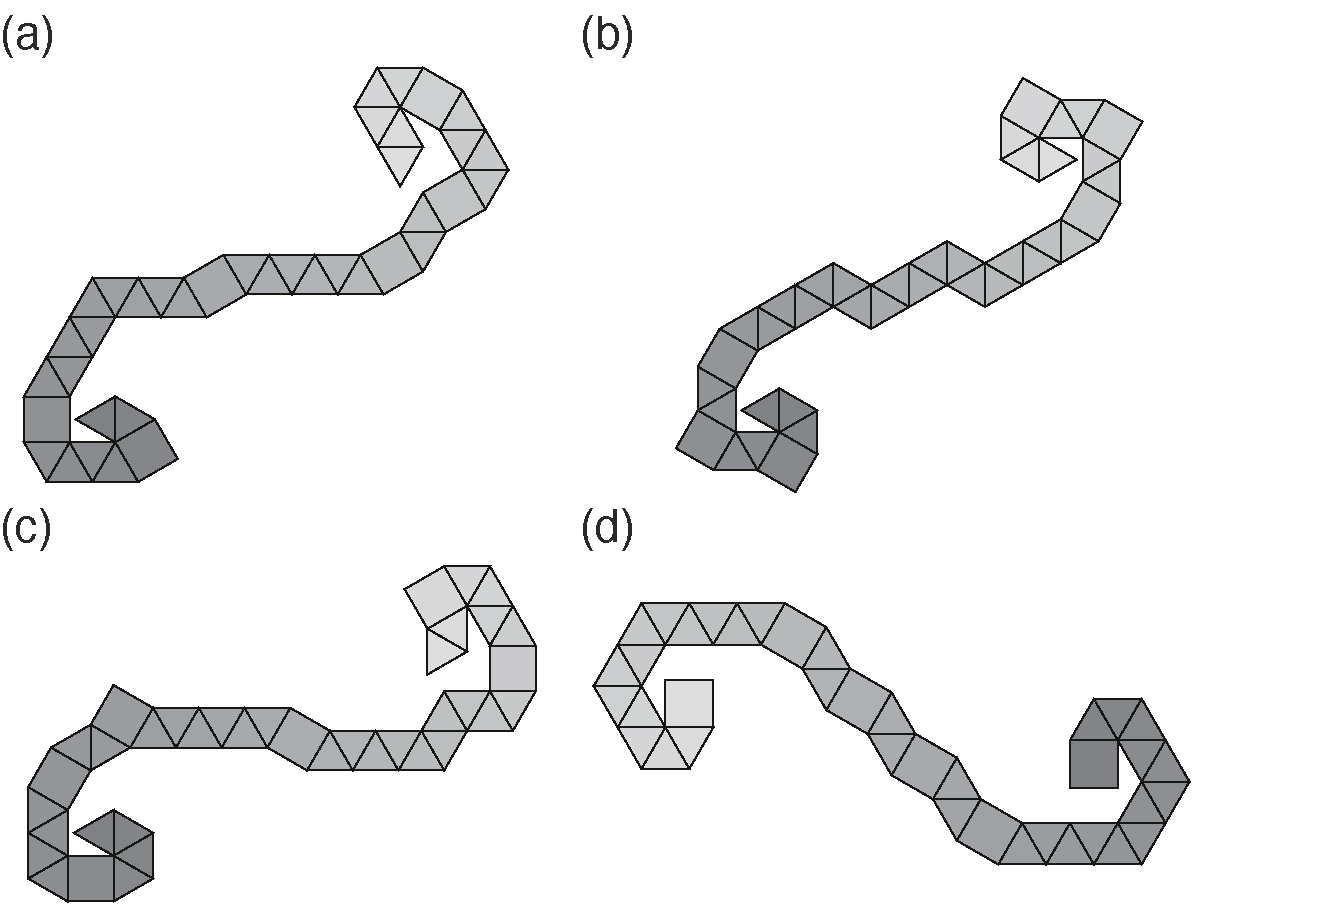
\includegraphics[width=\textwidth]{snubCube.pdf}
\caption{Snub Cube (38 faces, RZ rule with fallback): one representative
  net per successful orbit type for each chirality.
  \emph{Original} (left-handed / laevorotatory, 48/120 pairs):
    coordinates taken directly from Mathematica's
    \texttt{PolyhedronData["SnubCube"]} (snub triangles arranged
    counter-clockwise when viewed from outside a square face);
    $F_1{=}\text{snub}\,\triangle$ and $F_1{=}\text{gyrate}\,\triangle$.
  \emph{Mirror} (right-handed / dextrorotatory, 48/120 pairs):
    mirror image of the original (x-coordinates negated);
    $F_1{=}\text{snub}\,\triangle$ and $F_1{=}\square$.
  The square-starting orbit succeeds only for one chirality;
  the two enantiomers share the snub-triangle orbit but have otherwise
  disjoint successful orbit types.
  Color encodes selection order: dark gray (first face)
  $\to$ light gray (last face).}
\label{fig:snub-nets}
\end{figure}

The orbit-exchange behavior under mirror symmetry further confirms that
the algorithm is sensitive to chirality at the orbit level.
Table~\ref{tab:snub-orbits} shows the breakdown by orbit type under RZ
for both the original and the mirror image.

\begin{table}[ht]
\centering
\caption{Success counts by orbit type for the Snub Cube under RZ
  (original and mirror image).}
\label{tab:snub-orbits}
\renewcommand{\arraystretch}{1.15}
\begin{tabular}{lccc}
\toprule
$(F_1\text{-type},\,F_2\text{-type})$ & $n$ & Original & Mirror \\
\midrule
$\{\mathrm{snub},\mathrm{snub}\}$   & 24 & 24/24 & 24/24 \\
$\{\mathrm{gyrate},\mathrm{snub}\}$ & 24 & 24/24 & \ 0/24 \\
$\{\mathrm{sq},\mathrm{snub}\}$     & 24 & \ 0/24 & 24/24 \\
$\{\mathrm{snub},\mathrm{gyrate}\}$ & 24 & \ 0/24 & \ 0/24 \\
$\{\mathrm{snub},\mathrm{sq}\}$     & 24 & \ 0/24 & \ 0/24 \\
\bottomrule
\end{tabular}
\end{table}

The $\{\mathrm{snub},\mathrm{snub}\}$ orbit (24 pairs) succeeds under
both left and right spirals.
The orbit $\{\mathrm{gyrate},\mathrm{snub}\}$ succeeds only under the
original (right spiral), while $\{\mathrm{sq},\mathrm{snub}\}$
succeeds only under the mirror (left spiral).
These two orbits are exchanged by the reflection, reflecting the
geometric fact that gyrate triangles and square faces occupy
antipodally complementary roles in the two enantiomorphs.
The equal orbit sizes (24 each) explain why the total count is identical
despite the different sets of successful pairs.
This behavior confirms that the algorithm correctly distinguishes the two
enantiomorphs of the snub cube, even though the global count is preserved.

\clearpage
% ============================================================
\section{Extension to Four Dimensions}
\label{sec:4d}
% ============================================================

\subsection{4D Algorithm}

A 4-polytope is represented by vertex coordinates in $\mathbb{R}^4$,
a list of 2-faces (polygons), and a list of 3-cells
(polyhedra given as lists of face indices).
Two cells are \textbf{adjacent} if they share at least one face.

The peeling axis is the $w$-axis.
The algorithm rotates the polytope so that the centroid of the starting
cell $C_1$ aligns with the $+w$ direction; we call this orientation
\textbf{cell-centroid-up}, the 4D analogue of the 3D Face-up rotation.
The algorithm then proceeds as in the 3D case with cells replacing
faces and $w$ replacing $z$.
An alternative orientation, \textbf{3D-face-centroid-up}, aligns
$+w$ with the centroid of the shared 2-face between $C_1$ and a
chosen neighbor; this variant was computed for the 120-cell only,
and the results are presented in Section~\ref{sec:ex-120cell}.
The enumeration of nets of regular convex polytopes in dimension $\le 4$
was studied by Buekenhout and Parker~\cite{Buekenhout1998};
unfoldings and nets of regular polytopes are further explored
in~\cite{Devadoss2022}.

We employ the global $\mathbf{c}_1$--$\mathbf{c}_2$ determinant condition,
the direct 4D analogue of the 3D condition~\eqref{eq:left}:
\begin{equation}
  \det(\mathbf{c}_1,\,\mathbf{c}_2,\,\mathbf{c}_k,\,\mathbf{c}_j) \;\ge\; -\varepsilon,
  \quad \varepsilon = 10^{-10},
  \label{eq:4dleft}
\end{equation}
using a fixed global reference pair $(\mathbf{c}_1, \mathbf{c}_2)$.
Because $A\in\mathrm{SO}(4)$ satisfies $\det(A)=1$, the condition is
equivariant under the polytope's symmetry group.
We test both selection rules in this setting:
\begin{description}[nosep]
  \item[RZ (Zonal rule)] Primary: max $w$; secondary tie-break: max
    $\det(\mathbf{c}_1,\mathbf{c}_2,\mathbf{c}_k,\mathbf{c}_j)$.
    Fallback: min $w$, secondary max $|\det|$.
  \item[RS (Spiral rule)] Primary: max
    $\det(\mathbf{c}_1,\mathbf{c}_2,\mathbf{c}_k,\mathbf{c}_j)$;
    secondary tie-break: max $w$.
    Fallback: max $|\det|$, secondary min $w$.
\end{description}
Note that the 4D RS criterion is \emph{max} det, whereas the 3D RS
criterion is \emph{min} det (Section~\ref{sec:rules}).
This sign difference reflects the opposite orientation of the two
filter conditions: the 3D filter admits candidates with
$\det\le\varepsilon$ (negative side), so min det selects the most
extreme candidate in the filtered direction; the 4D filter admits
$\det\ge-\varepsilon$ (positive side), so max det plays the
analogous role.
At step $k=2$ the repeated row $\mathbf{c}_k=\mathbf{c}_2$ forces
$\det=0$, so the geometric score degenerates to the signed
$xy$-area $\mathbf{c}_{2,x}\mathbf{c}_{j,y}-\mathbf{c}_{2,y}\mathbf{c}_{j,x}$ at that step.
The same $xy$-area fallback is used at $k\ge 3$ whenever all candidate
determinants satisfy $|\det|<\varepsilon$.
Algorithm~\ref{alg:peel4d} gives the complete procedure.

\begin{algorithm}[tp]
\caption{Apple-Peel Unfolding (4D, global $\mathbf{c}_1$--$\mathbf{c}_2$ reference,
         rule $r\in\{\text{RS},\text{RZ}\}$,
         variant $v\in\{\text{w},\text{n}\}$).
         Variant w = with fallback; variant n = no fallback.}
\label{alg:peel4d}
\begin{algorithmic}[1]
\Require vertex coordinates, cells, adjacency lists,
         starting pair $(C_1,C_2)$, rule $r$, variant $v$,
         tolerance $\varepsilon=10^{-10}$
\Ensure cell selection order, success flag
\State Rotate (cell-centroid-up) so that $\mathbf{c}_{C_1}$ aligns with $+w$
\State $\mathit{order} \gets [C_1,\,C_2]$;\;
       $\mathit{last} \gets C_2$;\; $k \gets 2$
\While{$\mathit{last}$ has unvisited adjacent cells}
  \State $P \gets$ unvisited neighbors of $\mathit{last}$
  \If{$k = 2$}
    \State $R \gets P$;\quad
           $\mathit{score}(j) \gets \mathbf{c}_{2,x}\mathbf{c}_{j,y}-\mathbf{c}_{2,y}\mathbf{c}_{j,x}$
           \hfill ($xy$ cross product)
  \Else
    \State $R \gets \{\,j\in P : \det(\mathbf{c}_1,\mathbf{c}_2,\mathbf{c}_{\mathit{last}},\mathbf{c}_j)\ge -\varepsilon\,\}$
    \If{$\max_{j\in P}|\det(\mathbf{c}_1,\mathbf{c}_2,\mathbf{c}_{\mathit{last}},\mathbf{c}_j)| < \varepsilon$}
      \State $\mathit{score}(j) \gets \mathbf{c}_{2,x}\mathbf{c}_{j,y}-\mathbf{c}_{2,y}\mathbf{c}_{j,x}$
             \hfill (degenerate: $xy$ cross product)
    \Else
      \State $\mathit{score}(j) \gets \det(\mathbf{c}_1,\mathbf{c}_2,\mathbf{c}_{\mathit{last}},\mathbf{c}_j)$
    \EndIf
  \EndIf
  \If{$R \neq \emptyset$}
    \If{$r = \text{RZ}$}
      \State $\mathit{next} \gets \arg\max_{j\in R}(\mathbf{c}_j)_w$;\;
             $w$-ties broken by $\arg\max_j\,\mathit{score}(j)$
    \ElsIf{$r = \text{RS}$}
      \State $\mathit{next} \gets \arg\max_{j\in R}\,\mathit{score}(j)$;\;
             ties broken by $\arg\max_j\,(\mathbf{c}_j)_w$
    \EndIf
  \ElsIf{$v = \text{n}$} \Comment{no-fallback variant}
    \State \Return $(\mathit{order},\,\text{failure})$
  \Else \Comment{with-fallback variant: $R=\emptyset$, $v=\text{w}$}
    \If{$r = \text{RZ}$}
      \State $\mathit{next} \gets \arg\min_{j\in P}(\mathbf{c}_j)_w$;\;
             $w$-ties by $\arg\max_j\,|\mathit{score}(j)|$
    \ElsIf{$r = \text{RS}$}
      \State $\mathit{next} \gets \arg\max_{j\in P}|\mathit{score}(j)|$;\;
             ties by $\arg\min_j\,(\mathbf{c}_j)_w$
    \EndIf
  \EndIf
  \State append $\mathit{next}$ to $\mathit{order}$;\;
         remove $\mathit{next}$ from all adjacency lists;\;
         $\mathit{last} \gets \mathit{next}$;\; $k \gets k+1$
\EndWhile
\State \Return $\bigl(\mathit{order},\;|\mathit{order}|=|\mathit{cells}|\bigr)$
\end{algorithmic}
\end{algorithm}

\subsection{Results: Regular 4-Polytopes}
\label{sec:4dresults}

\begin{table}[ht]
\centering
\caption{Apple-Peel Unfolding with global $\mathbf{c}_1$--$\mathbf{c}_2$ reference.
  ``RZ'' = successful $(C_1,C_2)$ pairs under the Zonal rule;
  ``RS'' = successful pairs under the Spiral rule.
  Each successful pair produces a distinct cell-selection order;
  ``Class'' refers to RZ.}
\label{tab:4dglobal}
\renewcommand{\arraystretch}{1.2}
\begin{tabular}{lllrrrrl}
\toprule
Polytope & $\{p,q,r\}$ & Cell type & Cells & Total & RZ & RS & Class (RZ) \\
\midrule
5-cell   & $\{3,3,3\}$ & tetrahedron  &   5 &    20 &   20 &     20 & \textbf{Perfect}    \\
8-cell   & $\{4,3,3\}$ & cube         &   8 &    48 &   48 &     48 & \textbf{Perfect}    \\
16-cell  & $\{3,3,4\}$ & tetrahedron  &  16 &    64 &   20 &      0 & \textbf{Possible}   \\
24-cell  & $\{3,4,3\}$ & octahedron   &  24 &   192 &  192 &    192 & \textbf{Perfect}    \\
120-cell & $\{5,3,3\}$ & dodecahedron & 120 & 1{,}440 & 1{,}440 &      0 & \textbf{Perfect}    \\
600-cell & $\{3,3,5\}$ & tetrahedron  & 600 & 2{,}400 &      0 &      0 & \textbf{Impossible} \\
\bottomrule
\end{tabular}
\end{table}

\begin{remark}[Symmetry, orientation-sensitivity, and distinct net count]
\label{rem:symmetry}
For a regular polytope, the automorphism group acts transitively on
ordered adjacent cell pairs $(C_1, C_2)$.
The choice of pair affects the algorithm through two independent channels.
\begin{enumerate}[nosep,label=(\roman*)]
  \item \textbf{Cell-centroid-up orientation} (determined by $C_1$).
        The polytope is rotated so that $\mathbf{c}_{C_1}$ aligns with $+w$,
        fixing the coordinate system for all subsequent steps.
        Different choices of $C_1$ produce different rotations, changing
        the $w$-coordinates and $xy$-projections of every cell centroid.
  \item \textbf{Starting right condition} (determined by $C_2$).
        The right half-space filter uses the fixed reference plane
        spanned by $(\mathbf{c}_{C_1}, \mathbf{c}_{C_2})$
        (equation~\eqref{eq:4dleft}).
        Even when $C_1$ is fixed---and hence the coordinate system is
        unchanged---two different choices of $C_2$ define different
        reference planes, yielding different right-candidate sets at
        each step and potentially diverging selection sequences thereafter.
\end{enumerate}
Rules RS and RZ are sensitive to both channels, since they are defined
relative to the fixed $w$-axis and $xy$-plane.
A partial success rate (e.g.\ RZ achieves 20/64 on the 16-cell;
Table~\ref{tab:4dglobal})
therefore reflects the combined orientation-sensitivity of the rule,
not a combinatorial difficulty intrinsic to some starting pairs.

Regarding the distribution of $C_2$ choices: for a fixed $C_1$,
the number of $C_2$ candidates equals the number of faces of the cell
polyhedron---4 for the tetrahedral cells of the 5-cell, 16-cell, and 600-cell;
6 for the cubic cells of the 8-cell; 8 for the octahedral cells of the 24-cell;
and 12 for the dodecahedral cells of the 120-cell.
Unlike the 3D case---where the $C_p$ symmetry of the regular $p$-gon
face guarantees equal azimuthal spacing of $360^\circ/p$
(Remark~\ref{rem:symmetry3d})---the equal-spacing property does not
extend to 4D in general.
After cell-centroid-up alignment of $C_1$, the neighboring cell centroids lie
in the three-dimensional equatorial hyperplane ($w=0$) and project onto
the $xy$-plane in a pattern that depends on the specific geometry of the
cell polyhedron and its embedding; the azimuthal spacing is not
uniformly $360^\circ/n$ for $n$ choices.

For the \textbf{5-cell}, both RS and RZ achieve 20/20.
The automorphism group $\mathfrak{S}_5$ (order 120) acts transitively on
the 20 ordered adjacent pairs, and despite the two channels above,
the deterministic algorithm succeeds for every pair and produces a
single abstract cell-selection sequence up to the relabeling induced
by the automorphism.
Consequently, the 20 listed successes are 20 symmetry-equivalent instances
of one underlying unfolding; the number of geometrically distinct
3D nets is \textbf{one}.
(Verification that all 20 three-dimensional net realisations are congruent
is straightforward from the sorted pairwise-distance spectrum of the
vertex sets.)
\end{remark}

% ============================================================
\subsection{Three-Dimensional Realisation of 4D Unfoldings}
\label{sec:3dreal}
% ============================================================

Each successful cell-selection order can be realized as a
\emph{three-dimensional net} by embedding the cells of the 4-polytope
in $\mathbb{R}^3$ one at a time in selection order.
The procedure consists of three steps:

\begin{enumerate}[nosep]
  \item \textbf{SVD projection.}
        Each cell's vertices (in $\mathbb{R}^4$) are projected onto their
        best-fit 3-dimensional hyperplane via singular value decomposition,
        yielding an isometric local embedding.
  \item \textbf{Procrustes alignment.}
        The local embedding of each successive cell is aligned to the
        previous cell by minimizing the root-mean-square displacement of
        the shared-face vertices (rotation and translation only, no
        scaling).
        If the new cell and the previous cell end up on the same side of
        the shared face, a mirror reflection through that face is applied
        to place the new cell on the exterior side.
  \item \textbf{Overlap check.}
        All pairs of non-adjacent cells are tested for volumetric overlap
        using the Separating Axis Theorem (SAT) with face normals and
        edge cross-products as candidate axes; bounding-box pre-filtering
        is applied for efficiency.
        A tolerance $\varepsilon = 10^{-6}$ ensures that shared faces are
        not counted as overlaps.
\end{enumerate}

Algorithm~\ref{alg:net3d} formalises this procedure.

\begin{algorithm}[htbp]
\caption{3D Net Construction (4D polytopes)}
\label{alg:net3d}
\begin{algorithmic}[1]
\Require 4D vertex coordinates $\mathit{vers}$ (in $\mathbb{R}^4$),
         cell list (each cell as a list of face indices),
         selection order $[C_1,\ldots,C_m]$
\Ensure 3D vertex positions $\{\mathbf{q}[v]\}$, validity flag
\State \textbf{SVD projection of $C_1$:}
       find the best-fit 3-hyperplane of $C_1$'s vertices via SVD;
       set $\mathbf{q}[v]$ to the projected 3D coordinates for each
       $v\in C_1$
\For{$k \gets 2$ \textbf{to} $m$}
  \State \textbf{SVD projection of $C_k$:}
         project $C_k$'s 4D vertices onto $C_k$'s best-fit 3-hyperplane;
         let $\tilde{\mathbf{q}}[v]$ denote the local 3D coordinates
  \State $S \gets \text{shared face between } C_{k-1} \text{ and } C_k$
         \hfill\Comment{common 2-face}
  \State \textbf{Procrustes alignment:}
         find rotation $R$ and translation $\mathbf{t}$ minimising
         $\displaystyle\sum_{v\in S}
           \bigl\|\mathbf{q}[v]-(R\,\tilde{\mathbf{q}}[v]+\mathbf{t})\bigr\|^2$
  \State $\mathbf{q}[v] \gets R\,\tilde{\mathbf{q}}[v]+\mathbf{t}$
         for each $v\in C_k$
  \If{centroid of $C_k$ and centroid of $C_{k-1}$ lie on the \emph{same}
      side of face $S$}
    \State mirror-reflect all $\mathbf{q}[v]$ ($v\in C_k$) through the
           affine hyperplane of $S$
           \hfill\Comment{place $C_k$ on the exterior side}
  \EndIf
\EndFor
\State \textbf{Overlap check:}
       for each non-adjacent pair $(C_i,C_j)$, apply SAT with face
       normals and edge cross-products as separating-axis candidates
       (bounding-box pre-filter; tolerance $\varepsilon_{\mathrm{tol}}=10^{-6}$)
\State \Return $\bigl(\{\mathbf{q}[v]\},\;\text{all non-adjacent pairs separated}\bigr)$
\end{algorithmic}
\end{algorithm}

A realisation with no overlapping cells is called a
\textbf{valid 3D net}.
Table~\ref{tab:3dnet} summarizes the results for all successful
orderings produced by RZ (the best-performing rule).

\begin{table}[ht]
\centering
\caption{Three-dimensional net validity for the successful RZ orderings.
  ``Valid'' = no overlapping cell pairs under SAT\@.
  Dashes (---) for the 600-cell indicate no successful orderings
  (Impossible; see Table~\ref{tab:4dglobal}).}
\label{tab:3dnet}
\renewcommand{\arraystretch}{1.2}
\begin{tabular}{lrrrr}
\toprule
Polytope & Orderings & Valid & Overlap & Valid\,(\%) \\
\midrule
5-cell   &   20  &   20  &     0  & 100.0 \\
8-cell   &   48  &   48  &     0  & 100.0 \\
16-cell  &   20  &   20  &     0  & 100.0 \\
24-cell  &  192  &  192  &     0  & 100.0 \\
120-cell & 1440  &    0  &  1440  &   0.0 \\
600-cell &   —   &   —   &    —   &    —  \\
\bottomrule
\end{tabular}
\end{table}

\paragraph{Observations.}
\begin{itemize}[nosep]
  \item The 5-cell, 8-cell, 16-cell, and 24-cell yield \textbf{100\% valid nets}:
        every successful Apple-Peel ordering embeds without overlap in
        $\mathbb{R}^3$.
  \item The 120-cell produces \textbf{zero valid nets} despite yielding
        1440 successful 4D orderings.
        The dodecahedral cells are large relative to the overall
        assembly, and the long spiral path through 120 cells
        accumulates enough geometric distortion that self-intersection
        is unavoidable under the greedy strategy.
  \item The sharp transition from perfect 3D validity (5-, 8-, 16-, 24-cell)
        to zero validity (120-cell) suggests a combinatorial threshold
        related to cell size and the angular defect accumulated along
        the peel path.
\end{itemize}
Figure~\ref{fig:4d-nets} shows the resulting 3D nets for the four polytopes with valid realizations.

\begin{figure}[htbp]
\centering
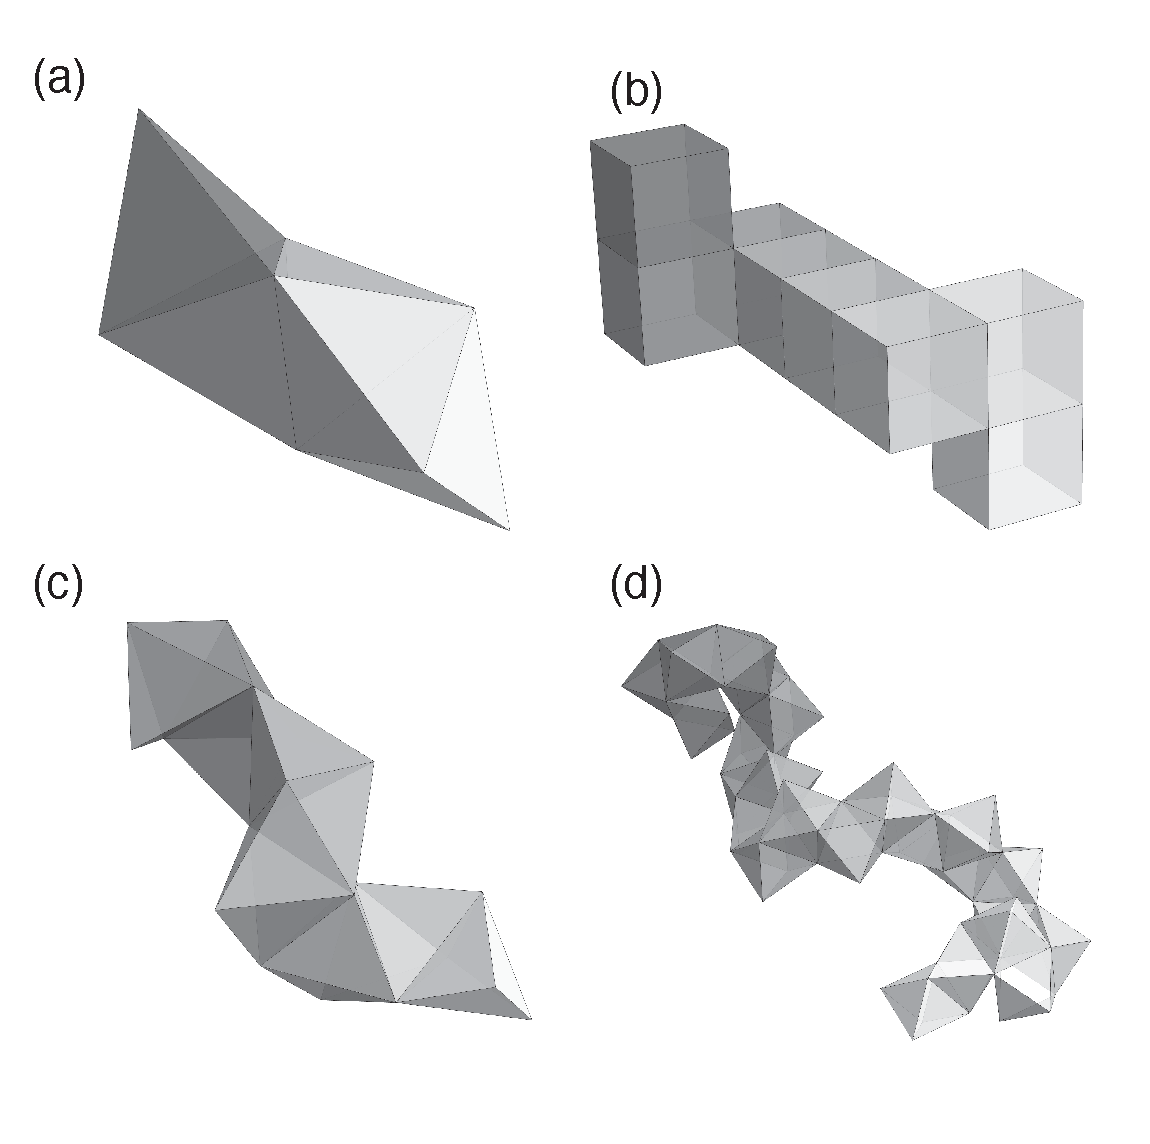
\includegraphics[width=\textwidth]{4d_nets.pdf}
\caption{Three-dimensional nets under Apple-Peel unfolding (RZ rule):
  (a)~5-cell, (b)~8-cell, (c)~16-cell, (d)~24-cell.
  For each polytope the net geometry is unique: all successful
  $(C_1,C_2)$ orderings yield congruent 3D shapes
  (verified computationally for all four polytopes).
  For the 5-cell, 8-cell, and 24-cell every ordering succeeds
  (Perfect); for the 16-cell, 20 of the 64 pairs succeed (Possible),
  and all successful orderings realize the same shape shown.
  Each net has no cell overlap (Table~\ref{tab:3dnet}).
  Color encodes selection order: dark gray (first cell)
  $\to$ light gray (last cell).}
\label{fig:4d-nets}
\end{figure}

\clearpage
% ============================================================
\section{Computational Examples}
\label{sec:examples}
% ============================================================

\subsection{Cross-Dimensional Summary}
\label{sec:crossdim}

Table~\ref{tab:summary} consolidates the
Perfect/Possible/Impossible classification
(defined in Section~\ref{sec:3d}) across all objects studied.

\begin{table}[ht]
\centering
\caption{Classification by best rule.
  4D results use the global $\mathbf{c}_1$--$\mathbf{c}_2$ reference;
  ``Best\,\%'' shows the success rate of the better rule for each
  solid (RZ in all cases except the truncated tetrahedron, where
  RS is better);
  see Table~\ref{tab:4dglobal} for the RS vs.\ RZ comparison.}
\label{tab:summary}
\renewcommand{\arraystretch}{1.2}
\begin{tabular}{lrrl}
\toprule
Object & Best rule & Best\,\% & Class \\
\midrule
\multicolumn{4}{l}{\textit{3D Platonic solids}} \\
Tetrahedron  & any & 100.0 & Perfect \\
Cube         & any & 100.0 & Perfect \\
Octahedron   & any & 100.0 & Perfect \\
Dodecahedron & any & 100.0 & Perfect \\
Icosahedron  & any & 100.0 & Perfect \\
\multicolumn{4}{l}{\textit{3D Archimedean solids (vertex config.)}} \\
Truncated Octahedron (4.6.6)         & RZ & 100.0 & Perfect \\
Truncated Icosahedron (5.6.6)        & RZ & 100.0 & Perfect \\
Truncated Cuboctahedron (4.6.8)      & RZ & 100.0 & Perfect \\
Truncated Icosidodecahedron (4.6.10) & RZ &  66.7 & Possible \\
Snub Cube (3.3.3.3.4)                & RZ &  40.0 & Possible \\
Truncated Tetrahedron (3.6.6)        & RS &  66.7 & Possible \\
7 remaining solids                   & -- &   0.0 & Impossible \\
\multicolumn{4}{l}{\textit{4D regular polytopes (global $\mathbf{c}_1$--$\mathbf{c}_2$ reference)}} \\
5-cell   & RZ & 100.0 & Perfect \\
8-cell   & RZ & 100.0 & Perfect \\
16-cell  & RZ &  31.3 & Possible \\
24-cell  & RZ & 100.0 & Perfect \\
120-cell & RZ & 100.0 & Perfect \\
600-cell & --  &   0.0 & Impossible \\
\bottomrule
\end{tabular}
\end{table}

We illustrate the algorithm's behavior on three representative
regular 4-polytopes.
Each example is parametrized by the starting pair $(C_1, C_2)$
and the resulting cell-selection sequence.

% ------------------------------------------------------------
\subsection{5-Cell: Agreement of RS and RZ}
\label{sec:ex-5cell}
% ------------------------------------------------------------

The 5-cell (pentachoron), the simplest regular 4-polytope with 5
tetrahedral cells, achieves a perfect result (20/20 pairs) under both
rules.
For every starting pair, both RS and RZ select the same complete
sequence through all 5 cells.
This agreement reflects the high symmetry of the 5-cell:
every pair of adjacent cells is equivalent under the automorphism group,
so the tiebreaking criterion used by each rule is never invoked in a
way that distinguishes one rule from another.
As noted in Remark~\ref{rem:symmetry}, the 20 successful pairs are all
symmetry-equivalent instances of this single sequence, and the resulting
3D realisations are all congruent---there is essentially one 5-cell net.
Kaino \cite{Kaino2019} reports the same results for the 5-cell,
8-cell, 16-cell, and 24-cell using a related spiral unfolding method.

% ------------------------------------------------------------
\subsection{16-Cell: RZ Stalling}
\label{sec:ex-16cell}
% ------------------------------------------------------------

The 16-cell (hexadecachoron) has 16 tetrahedral cells with 4 neighbors
each (64 pairs total).
RZ succeeds on 20 pairs (31.3\%) and RS is Impossible (0/64).
On a representative failing pair, RZ stalls after placing 15 of the
16 cells: the remaining cell is not adjacent to the last chosen cell.
The fully tetrahedral structure of the 16-cell (only 4 neighbors per
cell) creates a tight combinatorial constraint that the max-$w$
criterion cannot navigate for all starting pairs.

% ------------------------------------------------------------
\subsection{120-Cell: Perfect Result under RZ}
\label{sec:ex-120cell}
% ------------------------------------------------------------

The 120-cell (hecatonicosachoron) has 120 dodecahedral cells with
12 neighbors each (1,440 pairs total).
RZ achieves a Perfect result (1,440/1,440, 100\%) under the global
$\mathbf{c}_1$--$\mathbf{c}_2$ reference, while RS is Impossible (0/1,440).

For every starting pair the algorithm completes all 120 cells.
Although the primary criterion is max-$w$, the actual traversal path
is not a simple monotone band-by-band descent; the algorithm
repeatedly transitions between adjacent bands, zigzagging across
band boundaries throughout the 119-step sequence.
Each cell has 12 neighbors, providing enough connectivity for the
determinant-based right-half-space condition to always admit at least
one valid candidate or for the fallback (min-$w$) to bridge between
bands.
By contrast, RS (max-det primary) fails completely on the 120-cell,
reflecting the difficulty of maintaining a consistent spiral direction
in the densely connected dodecahedral structure.

\paragraph{Latitude-band structure.}
After cell-centroid-up rotation, the 120 cells arrange into
\textbf{9 bands} (grouped by symmetry orbit) numbered from the south
pole ($w$ smallest) to the north pole ($w$ largest, where $C_1$ resides):
\[
  \underbrace{1}_{\text{band 1}} + 12 + 20 + 12 + 30 + 12 + 20 +
  \underbrace{12}_{\text{band 8}} +
  \underbrace{1}_{\text{band 9}} = 120,
\]
with the 12 cells of $C_2$ candidates all residing in band~8
(directly adjacent to $C_1$ in band~9),
confirming that max-$w$ selection at step~$k=2$
is always a tie broken by the $xy$-cross-product score.
The 30-cell equatorial band ($w=0$) is the largest; the fallback
(min-$w$) is essential for bridging this band when the right-half-space
condition excludes all forward candidates.

\paragraph{Geometric diversity of RZ nets.}
Although all 1,440 cell-centroid-up orderings succeed, they do not
produce 1,440 distinct net shapes.
For fixed $C_1=3$ there are 12 adjacent $C_2$ choices, each yielding
a successful ordering, but geo-uniqueness testing
(pairwise centroid distances of the 3D embedding, rounded to $10^{-3}$)
reveals only \textbf{7 geometrically distinct net shapes}, grouped into
orbits $\{1,15,17,97\}$ (size~4), $\{4,18,51\}$ (size~3), and five
singletons $\{2\},\{10\},\{19\},\{100\},\{115\}$.

All 7 nets share a \emph{universal inner core}: the 3D distances
$r_{3D}$ of cell centroids in peeling order are identical for positions
$k=1,\ldots,13$ (the starting cell plus its 12 direct neighbors),
namely $r_{3D}\approx(0,\,1.70,\,1.79,\,1.80,\,1.81,\,1.82,\,1.81,
\,1.96,\,1.99,\,2.04,\,2.06,\,2.02,\,2.09)$.
The nets diverge only from $k=14$ onward.

Computing cylindrical coordinates $(r_{xy},z,\theta)$ of cell centroids
in the unfolded 3D net and summing the incremental turning angle reveals
three spiral-pattern types:
\begin{itemize}
  \item \textbf{Type A (CCW ascending)}: 5 of 7 nets wind counter-clockwise
    (positive total winding $+0.75$ to $+1.08$ turns), with $z$ increasing
    overall.  This is consistent with RZ's max-$xy$-cross-product
    tie-breaker, which preferentially selects cells in the
    counter-clockwise direction.
    Representative: $C_2=1$ ($+1.07$ turns, $z$: $-3$ to $+26$);
    also $C_2=10,19,100,115$.
  \item \textbf{Type B (CW / reversed)}: $C_2=2$ winds clockwise
    ($-1.14$ turns, $z$: $-7$ to $+4$).
  \item \textbf{Type C (near-zero / columnar)}: $C_2=4$ has nearly
    zero net winding ($-0.07$ turns) with $z$ spanning $-4$ to $+23$,
    producing a column-like rather than spiral structure.
\end{itemize}
Antipodal $C_2$ pairs (sharing opposite poles of the $C_1$ icosahedron:
$\{1,18\}$, $\{2,17\}$, $\{4,19\}$, $\{10,115\}$, $\{15,100\}$, $\{51,97\}$)
never share a geometric orbit, consistent with the $k=2$
tie-breaker reversing sign for antipodal choices.
Figure~\ref{fig:120cell-unfold} shows two representative nets contrasting the dominant CCW spiral and the columnar structure.

\begin{figure}[htbp]
\centering
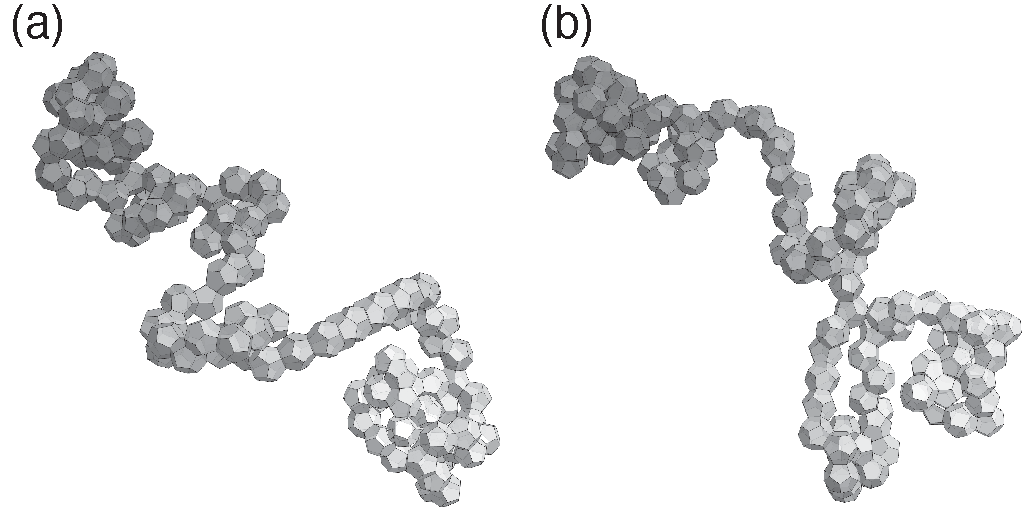
\includegraphics[width=0.85\textwidth]{120cell_unfolding.pdf}
\caption{Two representative three-dimensional nets of the 120-cell
  under RZ with fallback ($C_1=3$, 120/120 cells), chosen to
  contrast the two most distinct spiral-pattern types among the
  7 geo-unique net shapes.
  \emph{Left} (a): Type~A --- CCW spiral ($+1.07$ turns,
  $z\in[-3,+26]$), the dominant pattern (5 of 7 geo-unique nets).
  \emph{Right} (b): Type~C --- near-zero winding ($-0.07$ turns,
  $z\in[-4,+23]$), a qualitatively different columnar structure.
  Color encodes selection order: dark gray (first cell)
  $\to$ light gray (last cell).
  Both realisations self-intersect in 3D space; no non-overlapping
  net exists for the 120-cell under this algorithm.}
\label{fig:120cell-unfold}
\end{figure}

Kaino \cite{Kaino2019} also studies the 120-cell but treats it by
examining its layer structure separately, an approach that differs
from our greedy Apple-Peel algorithm.

\paragraph{Structure of self-intersections.}
To understand why all 120-cell nets self-intersect, we examined
whether overlapping cell pairs belong to the same latitude band
or to different bands.
For all 12 orderings with $C_1=3$ (308 total overlap pairs),
71.4\% of overlaps occur between cells in \emph{different} bands,
while only 28.6\% occur within the same band.
Moreover, the cross-band overlaps are almost exclusively between
\emph{adjacent} bands ($k \leftrightarrow k{+}1$); overlaps between
non-adjacent bands account for only a handful of cases.
This indicates that the self-intersections arise at band boundaries:
as each successive latitude band is unfolded into 3D space,
its dodecahedral cells protrude slightly into the region already
occupied by the preceding band, rather than distant bands
colliding directly.

\paragraph{3D-face-centroid-up orientation.}
We tested whether replacing cell-centroid-up with
\emph{3D-face-centroid-up}---aligning $+w$ with the centroid of
the shared pentagon between $C_1$ and a neighbor, the direct
4D analogue of the 3D Face-up rotation---reduces overlaps.
For 7 of the 12 adjacent $C_2$ choices ($C_1=3$), peeling
completes with an average of 18.6 overlapping pairs
(vs.\ 24.6 under cell-centroid-up for the same 7 pairs, a $\approx$24\% reduction);
the remaining 5 pairs fail to complete entirely.
No valid non-overlapping 3D net is obtained under either orientation,
confirming that the self-intersection of 120-cell nets is structural
rather than an artifact of the initial alignment.

\clearpage
% ============================================================
\section{Discussion}
\label{sec:discussion}
% ============================================================

Across both dimensions, high success rates correlate with
\textbf{uniform face types}.
Platonic solids and the 4D analogues (5-cell, 8-cell) with identical
cells perform best.
Solids with mixed face types---square-containing Archimedean solids
and the 600-cell---show low or zero rates.
The 120-cell is an exception: despite its complex dodecahedral cells it
achieves a Perfect result under RZ (100\%), owing to the high connectivity
(12 neighbors per cell) that keeps the determinant-based filter from
blocking all candidates.

\subsection{Spiral vs.\ Zonal Strategy in Four Dimensions}

A striking feature of the 4D results is the asymmetry between RS and RZ.
While both rules agree on the 5-cell, 8-cell, and 24-cell, RS fails
completely on the 16-cell (0/64) and the 120-cell (0/1,440),
whereas RZ achieves Possible and Perfect results respectively.

The difference stems from the distinct nature of the two primary criteria.
RZ's max-$w$ criterion provides a \emph{global monotone descent}: at every
step, RZ moves towards the ``south pole'' of the $w$-axis, a direction that
is always well-defined and consistent throughout the traversal.
This monotonicity makes RZ robust to local dead-ends---when no right
candidate exists, the fallback (min-$w$) continues the southward descent.

RS's max-det criterion, by contrast, requires \emph{consistent spiral
curvature} relative to the fixed $\mathbf{c}_1$--$\mathbf{c}_2$ plane.
In 3D, the face-up rotation and the regular structure of Platonic solids
ensure that the spiral curvature is compatible with the right-half-space
filter at every step.
In 4D, however, the equatorial hyperplane ($w=0$) contains cell centroids
in a three-dimensional arrangement that reflects the geometry of the cell
polyhedron.
For the 120-cell, whose cells are regular dodecahedra, the 12 neighbors
of each cell form an icosahedral arrangement in the equatorial hyperplane.
The max-det criterion selects the candidate that maximizes signed
four-dimensional volume, but the icosahedral symmetry creates configurations
where the right-half-space filter and the max-det selection are mutually
incompatible: the filter admits only candidates whose determinant is
near zero, and among those, max-det provides no meaningful ordering.
The result is systematic failure.
RZ avoids this by falling back to max-$w$, which resolves the degeneracy
via a globally consistent criterion.

The 600-cell is Impossible under both RZ and RS.
Despite having only 4 neighbors per cell (the same as the 16-cell, which
is Possible under RZ), the 600 tetrahedral cells create a combinatorial
structure that no greedy rule can traverse completely.
Analysis of the termination-step distribution reveals that all 2\,400
evaluated $(C_1, C_2)$ pairs halt at one of exactly five step values
(146, 150, 276, 279, or 284), indicating structural bottlenecks related
to the 600-cell's icosahedral symmetry.
We further tested one-step backtracking, 3D-face-centroid-up orientation,
and vertex-up orientation; all variants remain Impossible,
confirming that the obstacle is structural rather than an artifact
of the specific greedy heuristic or orientation choice.
The low per-cell connectivity (4 neighbors) means that the
determinant-based right-half-space condition can simultaneously exclude
all remaining candidates, a situation that does not arise for the
120-cell (12 neighbors per cell).
Kaino \cite{Kaino2019} also studies the 600-cell using a layer-based
approach; both methods leave the 600-cell unresolved, but the
approaches differ.

\subsection{Relation to the Companion Implementation}

The algorithm implemented here differs in three respects from the
companion paper~\cite{Yoshino2026arXiv}.
First, the right-half-space filter there uses the \emph{current} face
centroid $\mathbf{c}_k$ as reference, with the strict condition
$(\mathbf{c}_k \times \hat{z})_{xy}\cdot\mathbf{c}_{j,xy}>0$,
rather than the global fixed reference $\mathbf{c}_1$ with tolerance
$\varepsilon$ adopted here.
Second, tie-breaking among candidates with equal $z$ resolves by list
order (first occurrence in the face-index sequence) rather than by the
equivariant min-Det criterion.
Third, the RS (min-Det) rule is new to the present paper; the companion
implements only max-$z$ selection.

The local reference and list-order tie-break implicitly break equivariance:
the filter direction rotates at every step, and tie outcomes depend on the
internal ordering of faces in the data structure.
Consequently, the companion implementation reports fractional success rates
for symmetric solids---for instance, 53.3\% for the dodecahedron---whereas
equivariance theory predicts all-or-nothing rates.
The global $\mathbf{c}_1$ reference, equivariant min-Det tie-break, and
$\varepsilon$-threshold adopted here restore equivariance and are more
robust to floating-point rounding.

% ============================================================
\section{Conclusion}
% ============================================================

We evaluated two Apple-Peel Unfolding rules (RS, RZ) on 24 objects
across two dimensions.
The main findings are:
\begin{enumerate}
  \item \textbf{RZ dominates in 4D.}
        Under the global $\mathbf{c}_1$--$\mathbf{c}_2$ reference algorithm, RZ achieves
        Perfect on the 5-cell, 8-cell, 24-cell, and \textbf{120-cell} (100\%),
        and Possible on the 16-cell (31.3\%).
        RS is Impossible on the 16-cell and 120-cell, and matches RZ only
        on the 5-cell, 8-cell, and 24-cell.
  \item \textbf{RZ achieves 100\%} on three of thirteen Archimedean
        solids (truncated octahedron, truncated icosahedron, truncated
        cuboctahedron), and 66.7\% on the truncated icosidodecahedron;
        the snub cube and truncated tetrahedron yield partial success
        (RZ 40\% and RZ 33.3\%, respectively);
        seven of thirteen remain Impossible under both rules.
  \item \textbf{RZ outperforms RS on these four solids}:
        truncated octahedron (100\% vs.\ 41.7\%),
        truncated cuboctahedron (100\% vs.\ 0\%),
        truncated icosahedron (100\% vs.\ 0\%),
        truncated icosidodecahedron (66.7\% vs.\ 0\%).
        The sole case where RS outperforms RZ is the
        \textbf{truncated tetrahedron} (RS 66.7\% vs.\ RZ 33.3\%).
  \item The 600-cell and seven Archimedean solids are Impossible;
        impossibility correlates with structural non-uniformity or
        high combinatorial complexity.
        The 600-cell terminates at one of five fixed steps for all pairs,
        indicating icosahedral bottlenecks.
\end{enumerate}

Future work includes investigating two-stage selection strategies
(e.g.\ RZ followed by RS as a tiebreaker),
extending the valid-net analysis to characterize which
Apple-Peel orders produce non-overlapping three-dimensional nets,
and applying both rules to random convex polyhedra---for example,
convex hulls of random point sets---to assess how success rates
and overlap frequency vary with combinatorial structure
beyond the symmetric cases studied here.

% ============================================================
\section*{Acknowledgements}
% ============================================================

One of the authors (T.Y.) thanks Prof.\ Keimei Kaino, emeritus professor
of the National Institute of Technology Sendai College,
for comments on the results during the preparation of the manuscript.
This work was supported in part by the Inoue Grant of Toyo University.
This research also received funding through the Toyo University
Short-term International Visiting Professor Program in 2022,
and partial support from Chiang Mai University.

% ============================================================
\begin{thebibliography}{9}
% ============================================================

\bibitem{Shephard1975}
G.~C.~Shephard,
Convex polytopes with convex nets,
\textit{Math.\ Proc.\ Cambridge Philos.\ Soc.},
\textbf{78} (1975), 389--403.

\bibitem{Demaine2007}
E.~D.~Demaine and J.~O'Rourke,
\textit{Geometric Folding Algorithms: Linkages, Origami, Polyhedra},
Cambridge University Press, 2007.

\bibitem{AronovORourke1992}
B.~Aronov and J.~O'Rourke,
Nonoverlap of the star unfolding,
\textit{Discrete Comput.\ Geom.},
\textbf{8} (1992), 219--250.

\bibitem{Lubiw2010}
A.~Lubiw, E.~D.~Demaine, M.~L.~Demaine, A.~Schwartz, and J.~Snoeyink,
Zipper unfoldings of polyhedral complexes,
in \textit{Proc.\ 22nd Canadian Conf.\ Comput.\ Geom.\ (CCCG 2010)},
219--222.

\bibitem{ORourke2015}
J.~O'Rourke,
Spiral unfoldings of convex polyhedra,
arXiv:1509.00321, 2015.

\bibitem{Buekenhout1998}
F.~Buekenhout and M.~Parker,
The number of nets of the regular convex polytopes in dimension $\leq 4$,
\textit{Discrete Math.},
\textbf{186} (1998), 69--94.

\bibitem{Devadoss2022}
S.~Devadoss and M.~Harvey,
Unfoldings and nets of regular polytopes,
\textit{Comput.\ Geom.: Theory Appl.}\ (2022).
arXiv:2111.01359.

\bibitem{Akitaya2024}
H.~A.~Akitaya, R.~Samanta, et al.,
Path-unfolding the tesseract,
\textit{Fall Workshop on Computational Geometry (FWCG 2024)}.

\bibitem{Yoshino2026arXiv}
T.~Yoshino and S.~Chaidee,
Apple peel unfolding of {A}rchimedean and {C}atalan solids,
arXiv:2604.16204, 2026.

\bibitem{Kaino2019}
K.~Kaino,
Apple-peel foldouts of four-dimensional regular polytopes:
24, 120 and 600-cells,
\textit{Symmetry: Art and Science},
\textbf{2019}, No.~1--4, 142--145.

\end{thebibliography}

\end{document}
